\chapter{NeedFinding}

La prima parte del nostro lavoro, denominato come \textit{NeedFinding},
si è basato su due fasi:
\begin{enumerate}
    \item \textbf{Interviste}
    \item \textbf{Questionario}
\end{enumerate}
Con quest'ultime si è cercati di delineare i \textit{Needs} (bisogni)
e i possibili \textit{Task} degli utenti relativi all'applicazione.\\

L'obiettivo delle nostre interviste è quello di ottenere una visione completa e diversificata delle esigenze degli studenti di Sapienza nello gestire la vita accademica.
Per ottenere questa panoramica ampia e rappresentativa abbiamo intervistato studenti di vari dipartimenti in Sapienza, con diversi livelli di istruzione, e di età e background culturali differenti.
A questo fine la maggior parte delle interviste è stata condotta all'interno dell'ateneo stesso.

\section{Interviste}
Il primo passaggio da fare, come consueto nel needfinding, è 
determinare le domande per le interviste degli utenti. 
La stesura delle domande è basato su tre macrotemi riguardanti 
i bisogni degli studenti:
\begin{itemize}
    \item \textbf{Percorso Formativo}
    \item \textbf{Opinione riguardo i Professori}
    \item \textbf{Tirocinio}
\end{itemize}
La formulazione delle domande per le interviste sono poste in modo generico
per non convincere lo studente della nostra opinione, bensì per confermare 
che sia una necessità e che sia un bisogno di ogni singolo studente il parere dei 
propri colleghi riguardo ai professori affinché ci sia consapevolezza e chiarezza
nella scelta di un corso e/o di un tirocinio.


\subsection{Domande Interviste}
Le domande che abbiamo formulato sono le seguenti:
\subsubsection{Domande per Rompere il Ghiaccio}
\textcolor{darkblue}{\textbf{Motivazione:} Le \textit{Domande per Rompere il Ghiaccio} hanno la finalità
di mettere a proprio agio l'utente, mostrando interesse da parte nostra. 
In aggiunta, la prima domanda è utile a noi per determinare se fa parte del nostro target}
\begin{enumerate}
    \item Ciao, Come ti chiami? Quanti anni hai? Sei uno studente di Sapienza?
    \item Stai conseguendo una Laurea Triennale o Magistrale?
    \item Che corso di laurea stai conseguendo?  In che anno accademico ti sei iscritto?
\end{enumerate}

\subsubsection{Domande sul Percorso Formativo}
Nel tuo percorso formativo sai se sono previsti corsi a scelta?\\
\textcolor{darkblue}{\textbf{Motivazione:} Con questa prima domanda sul Percorso Formativo vogliamo distinguere chi si è informato a riguardo e chi no, 
così da poter porre domande idonee per i due casi ed escludere totalmente chi frequenta corsi che non prevedono esami a scelta}
\begin{itemize}
    \item \textbf{Se SI (quindi vuol dire che lo studente/ssa  sa che ci sono corsi a scelta e si è informato/a)}\\
    Se si, ti sei informato?\\
    Hai compilato il percorso formativo e ne stai già frequentando qualcuno?\\
    \textcolor{darkblue}{\textbf{Motivazione:} Identifichiamo due tipologie di user:
    \begin{enumerate}
        \item Gli studenti che sanno dei corsi a scelta ma non hanno ancora compilato il percorso formativo
        \item Gli studenti che sanno dei corsi a scelta e stanno frequentando/hanno concluso
    \end{enumerate}}
    \begin{itemize}
        \item \textbf{Se NO (quindi, studente che non ha ancora compilato il percorso formativo)}\\
        Hai già scelto i corsi?\\
        \textcolor{darkblue}{\textbf{Motivazione:} Un'ultima distinzione da dover fare è la seguente:
        \begin{enumerate}
            \item Chi non ha scelto corsi
            \item Chi ha più o meno un'idea di che corsi vorrà fare
        \end{enumerate}}
        
        \begin{itemize}
            \item \textbf{Se No: (Studente che non ha scelto i corsi)}
            \begin{enumerate}
                \item Perché?
                \item Descrivi gli step che faresti per cercare i tuoi futuri corsi
            \end{enumerate}
            \textcolor{darkblue}{\textbf{Motivazione:} Queste due domande ci aiutano a capire le motivazioni per cui non ha ancora compilato, ma sopratutto capire se i mezzi
            messi a disposizione da Sapienza (sitoweb) per la ricerca sono intituivi e chiari}

            \item \textbf{Se Si: (Studente che ha scelto i corsi, ossia che ha un’idea di che corsi vorrà fare)}\\
            Come hai reperito/ricercato i corsi? Possibile risposte:\\
            \textcolor{darkblue}{\textbf{Motivazione:} Poniamo questa domanda per ricercare la via di comunicazione più comune tra gli studenti. 
            Di esse, il team (rispetto alle proprie esperienze) ne ha evidenziate principalmente due: Passaparola, Catalogo Sapienza}

            \begin{itemize}
                \item \textbf{Passaparola (Consigliato Da)}
                \begin{enumerate}
                    \item Chi te l'ha consigliato?
                    \item Ti è stato utile il consiglio? Perché?
                \end{enumerate}
                \textcolor{darkblue}{\textbf{Motivazione:} Le due domande generiche poste qui sopra, hanno un ruolo fondamentale: Capire se la comunicazione tra studenti è un vero e proprio \textit{Need}}

                \item \textbf{Catalogo Sapienza}
                \begin{enumerate}
                    \item Descrivi gli step della ricerca dei corsi
                    \item Gli step erano chiari e intuitivi? (O si o no) Perché?\\
                    \textcolor{darkblue}{\textbf{Motivazione:} Vogliamo capire se il sito Sapienza riesce ad aiutare gli studenti a ricercare le informazioni riguardanti il corso da voler scegliere.}
                \end{enumerate}
                Cosa ricerchi nella descrizione del corso? Riesci a trovare queste informazioni nella tua ricerca?\\
                \textcolor{darkblue}{\textbf{Motivazione:} Dopo aver preso un po' di confidenza con l'utente, poniamo una domanda più personale per determinare gli interessi 
                effettivi di un corso; queste informazioni saranno poi utili per la creazione del questionario}
            \end{itemize}
            
        \end{itemize}

        \item \textbf{Se SI (Studente che ha compilato il percorso formativo (sia in corso che già concluso))}
        \begin{enumerate}
            \item Come hai trovato i corsi? Possibile risposte:
            \begin{itemize}
                \item \textbf{Passaparola}
                \begin{enumerate}
                    \item Chi te l'ha consigliato? Perché?
                    \item Ti è stato utile il consiglio? Perché?
                \end{enumerate}

                \item \textbf{Catalogo Sapienza}
                \begin{enumerate}
                    \item Descrivi gli step della ricerca dei corsi
                    \item Gli step erano chiari e intuitivi? (O si o no) Perché?
                \end{enumerate}
            \end{itemize}

            \item Cosa ricerchi nella descrizione del corso? Riesci a trovare queste informazioni nella tua ricerca?\\
            \textcolor{darkblue}{\textbf{Motivazione:} Le domande sopra sono uguali a quelle poste nel branch: \textit{Se Si: (Studente che ha scelto i corsi, ossia che ha un’idea di che corsi
            vorrà fare)}}
            \item Tornando indietro lo sceglieresti di nuovo? Perché? (Aggiunta: rimoduleresti il percorso formativo scegliendo altri corsi?)\\
            \textcolor{darkblue}{\textbf{Motivazione:} In questa domanda vogliamo capire se l'utente è stato soddisfatto della sua scelta, oppure no.
            Il \textit{Perché} dopo è utile soprattutto per un eventuale \textit{No} poiché, come motivazione della risposta, potrebbero emergere dei \textit{Need} interessanti}
            \item Avendo frequentato i corsi, la descrizione di quest'utltima corrisponde a quello che ti avevano descritto/letto sul sito prima di seguire le lezioni?(sia che scelto per sentito dire sia che tu abbia visto il sito)\\
            \textcolor{darkblue}{\textbf{Motivazione:} Avendo frequentato/ frequentando il corso vogliamo capire se le aspettative del mezzo con cui 
            si sono informati (Passaparola, Sitoweb) gli/le è stato utile. L'utilità di questa informazione per il team è di voler paragonare i due mezzi di comunicazione e
            cercare di capire quanto è più veritiero/autentico l'opinione dello studente rispetto ad una semplice descrizione del sito}
            \item Qualcuno ti ha chiesto dal vivo o online dei feedback o consigli riguardo al corso scelto.\\
            \textcolor{darkblue}{\textbf{Motivazione:} Indaghiamo ancora di più sulla comunicazione degli studenti riguardo ai corsi}  
        \end{enumerate}

    \end{itemize}
    
    \item \textbf{Se NO (l’utente non ha ancora scelto i corsi ma è consapevole di doverli scegliere)}
    \begin{enumerate}
        \item Perchė non li hai ancora scelti?
        \item Descrivi gli step che faresti per cercare i tuoi futuri corsi.
    \end{enumerate}

\end{itemize}

\subsubsection{Domande sulle Opinioni riguardo i Professori}
Parlando dell’insegnamento dei corsi, ti volevamo chiedere:
\begin{enumerate}
    \item Prima di iniziare un corso qualsiasi nel tuo percorso di studi ti interessa informarti del professore che terrà il corso?\\
    \textcolor{darkblue}{\textbf{Motivazione:} Vogliamo capire a primo impatto l'interesse dello studente riguardo il professore}
    \begin{itemize}
        \item \textbf{Se SI: (Studenti che si informano del professore)}
        \begin{enumerate}
            \item Descrivi le procedure che usi per informarti.
            \item Quali sono gli aspetti su cui ti informi riguardo al professore?\\
            \textcolor{darkblue}{\textbf{Motivazione:} Come abbiamo fatto nella sezione \textit{Percorso Formativo}, abbiamo posto una domanda più personale per determinare
            le informazioni principali per uno studente riguardo al professore; anche quest'ultime saranno poi utili per la creazione del questionario }
            \item \textbf{(Solo chi ha corsi ha scelta:)} Nel caso di un corso a scelta, l’informazione del professore hanno influito/possono influire alla scelta del corso?\\
            \textcolor{darkblue}{\textbf{Motivazione:} Accentuiamo ancora di più la ricerca degli aspetti fondamentali per la scelta dei corsi, ponendo un taglio riguardo alle informazioni del professore}
        \end{enumerate}
    
        \item \textbf{Se NO: (Studenti che non si informano del professore)}\\
        Perché?\\
        \textcolor{darkblue}{\textbf{Motivazione:} Capire se questa mancanza di informazioni è dovuto alla poca chiarezza del sito o poca comunicazione tra i colleghi}
    \end{itemize}

    \item Ti è semplice reperire il materiale dal professore ( sia quello utilizzato a lezione che quello al di fuori )?\\
    \textcolor{darkblue}{\textbf{Motivazione:} Un'esigenza di cui si è domandato il team riguardante il professore è il materiale a lezione.
    Con questa domanda vogliamo capire la reperibilità del professore riguardo ai materiali, e se sono disponibili per tutti}
    \begin{itemize}
        \item \textbf{Se SI:}
        \begin{enumerate}
            \item Ti capita di incrementare con fonti esterne?\\
            \textcolor{darkblue}{\textbf{Motivazione:} Vogliamo capire se è sufficiente la lezione o c'è una neccesità di reperire anche altro}
            \item I tuoi colleghi sono disponibili condividere il materiale?\\
            \textcolor{darkblue}{\textbf{Motivazione:} Con questa domanda vogliamo evidenziare la necessità o meno della comunicazione tra i colleghi. 
            Vogliamo capire se la comunicazione tra gli studenti è un \textit{Need}}
            \item Utilizzi la tecnica delle sbobbine?\\
            \textcolor{darkblue}{\textbf{Motivazione:} Questa domanda è stata aggiunta successivamente poiché dalle risposte degli utenti della domanda sopra è emersa
            la tecnica delle sbobbine}
        \end{enumerate}

        \item \textbf{Se NO:}
        \begin{itemize}
            \item Da dove prendi il materiale?
            \item \textbf{(Nel momento in cui ti risponde: i colleghi)} I tuoi colleghi sono disponibili a condividere il materiale?\\
            \textcolor{darkblue}{\textbf{Motivazione:} Capire se c'è un'esigenza sulla comunicazione tra gli studenti per quanto riguarda gli appunti}
        \end{itemize}
    \end{itemize}
\end{enumerate}

\subsubsection{Domande sul Tirocinio}
Passando all'argomento Tirocinio, è previsto un periodo di tirocinio nel tuo Corso di Laurea? Possibili risposte:\\
\textcolor{darkblue}{\textbf{Motivazione:} Identifichiamo il target di utenti con cui andiamo a fare domande più specifiche}
\begin{itemize}
    \item \textbf{NO: (Non esiste il tirocinio)}\\
    \textbf{Finito Intervista}: Buona giornata
    \item \textbf{Non lo so}\\
    \textbf{Finito Intervista}: Buona giornata
    \item \textbf{SI: (Esiste il Tirocinio e sa)}\\
    Ti sei informato a riguardo?\\
    \textcolor{darkblue}{\textbf{Motivazione:} Vogliamo capire l'interesse dello studente riguardo il tirocinio}
    \begin{itemize}
        \item \textbf{Se NO: (Non si è informato del Tirocinio)}\\
        Perché e Come pensi di informarti?\\
        \textcolor{darkblue}{\textbf{Motivazione:} Capire se questa mancanza di informazioni è dovuto alla poca chiarezza del sito od è semplicemeente disinteresse}
        \item \textbf{Se SI: (Si è informato del Tirocinio)}
        \begin{enumerate}
            \item Descrivi gli step di come ti sei informato
            \item Hai trovato questi step chiari e intuitivi?\\
            \textcolor{darkblue}{\textbf{Motivazione:} Vogliamo capire se il mezzo con cui si è informato (si pensa principalmente al sito Sapienza) riesce ad aiutare gli studenti a ricercare i tirocini in modo semplice e intuitivo.}
            \item Le informazioni trovate sul tirocinio (riguardante il tirocinio in sé) ti hanno permesso di avere una visione di questo chiara e completa?\\
            \textcolor{darkblue}{\textbf{Motivazione:} Poniamo questa domanda per capire se le informazioni sono state esaustive per la scelta di un possibile tirocinio 
            cercando di estrapolare in maniera indiretta i punti chiave di esso; quest’ultime saranno poi utili per la
            creazione del questionario }
            \item Sei a conoscenza che il tirocinio si può fare sia interno che esterno? Tu quale pensi di scegliere o hai scelto? Possibili risposte:\\
            \textcolor{darkblue}{\textbf{Motivazione:} Identifichiamo il target di utenti con cui andiamo a fare domande.
            Il nostro progetto mira sulle opinioni degli studenti riguardo ai professori, perciò ci interessa esaminare
            soltanto gli studenti che hanno svolto/stanno per svolgere/vogliono svolgere un tirocinio interno}
            \begin{itemize}
                \item \textbf{Esterno: (Non ci interessa)}\\
                \textbf{Finito Intervista}: Buona giornata
                \item \textbf{Interno:}\\
                Lo devi ancora fare o lo stai già frequentando/concluso? Possibili Risposte:
                \begin{itemize}
                    \item \textbf{BLOCCO 1: NO (Persona che non ha ancora iniziato)}
                    \item \textbf{BLOCCO 2: SI (Persona che l'ha già iniziato/ concluso)}
                \end{itemize}
            \end{itemize}
        \end{enumerate}
    \end{itemize}
\end{itemize}

\textbf{BLOCCO 1}\\
La scelta del professore con cui fare il tirocinio è indotta da te o da sapienza?\\
\textcolor{darkblue}{\textbf{Motivazione:} Vogliamo capire se la scelta del professore con cui fare il tirocinio è vincolato dalla scelta di Sapienza o c'è libertà dello studente
per porre domande più personali/soggettive a quest'ultimo target}
\begin{itemize}
    \item \textbf{Scelta Personale}
    \begin{enumerate}
        \item Come hai scelto il professore/ come pensi di sceglierlo?
        \item Hai delle condizioni che dovrebbero essere soddisfatte? Descrivi quali.\\
        \textcolor{darkblue}{\textbf{Motivazione:} Poniamo una domanda più personale per determinare le informazioni principali per
        uno studente riguardo alla scelta del professore per un tirocinio; anche quest’ultime saranno poi utili per la creazione del questionario}
        \item Le informazioni sul tirocinio del professore dove le hai trovate? erano chiare e esplicative?\\
        \textcolor{darkblue}{\textbf{Motivazione:} Questa domanda è utile al team per capire se c'è una necessità di migliorare il \textit{Task} di trovare le informazioni sul tirocinio}
        \item Pensi di contattarlo personalmente/ l'hai contattato personalmente? Cosa gli-le hai chiesto/vorresti chieder-le/gli in particolare?\\
        \textcolor{darkblue}{\textbf{Motivazione:} Avendo più confidenza con l'utente, abbiamo voluto porre una domanda più specifica su quali sono le sue esigenze per la scelta del professore}
        \item (Se l'ha contattato) È stato reperibile? È chiaro riguardo i tirocini da lui offerti?\\
        \textcolor{darkblue}{\textbf{Motivazione:} Per interessarci dell'utente cercando di non porre domande tutte pesanti, abbiamo pensato di voler mettere una domanda per raccontarci della sua esperienza 
        cercando magari di estrapolare altre informazioni utili}
        \item Hai ricevuto e/o ricercato consigli o opinioni da altri studenti?\\
        \textcolor{darkblue}{\textbf{Motivazione:} Vogliamo capire quanto ci sia la comunicazione tra studenti riguardante il Tirocinio e quanto possa influire}
        \begin{itemize}
            \item \textbf{Se si: (Ricevuto gli opinioni degli studenti)}\\
            Questi hanno influito nella scelta? Perché?\\
            \textcolor{darkblue}{\textbf{Motivazione:} Il tema del tirocinio può essere sicuramente centrale nella comunicazione tra gli studenti, vogliamo capire quanto per capire se può essere un \textit{Need}}
            \item \textbf{Se no: (Non Ricevuto opinioni)}\\
            Avresti voluto averne?\\
            \textcolor{darkblue}{\textbf{Motivazione:} Questa domanda ci può essere utile nel momento in cui lo studente non ha avuto i mezzi buoni per informarsi con studenti 
            che hanno fatto il tirocinio con quel professore}
        \end{itemize}
    \end{enumerate}
    \item \textbf{Scelto da Sapienza}\\
    Ti sei informato riguardo al professore?\\
    \textcolor{darkblue}{\textbf{Motivazione:} Capiamo se c'è interesse riguardo alle informazioni del professore}
    \begin{itemize}
        \item \textbf{Se SI:}
        \begin{itemize}
            \item Come hai trovato informazioni sul professore?
            \item Hai provato a contattarlo anche personalmente? Perché?
            
        \end{itemize}

        \item \textbf{Se NO:}\\
        \textbf{Finito Intervista}: Buona giornata
    \end{itemize}

\end{itemize}


\textbf{BLOCCO 2}\\
\textcolor{darkblue}{\textbf{Motivazione:} Le domande del BLOCCO 2 sono simili a quelle del BLOCCO 1
con l'unica differenza che abbiamo voluto capire se sono soddisfatti le informazioni che hanno ricercato (se hanno ricercato) prima di iniziare il tirocinio}\\
La scelta del professore con cui fare tirocinio è indotta da te o da sapienza?
\begin{itemize}
    \item \textbf{Scelta Personale}
    \begin{enumerate}
        \item Come hai scelto il professore?
        \item Avevi delle condizioni che dovevano essere soddisfatte?
        \begin{itemize}
            \item \textbf{Se SI:}
            \begin{enumerate}
                \item Descrivi cosa in particolare
                \item Pensi che siano state soddisfatte? Perché?
            \end{enumerate}
            \item \textbf{Se NO:}\\
            \textbf{Finito Intervista}: Buona giornata
        \end{itemize}
        \item Hai ricevuto consigli o opinioni da altri studenti?
        \begin{itemize}
            \item \textbf{Se si: (Ricevuto gli opinioni degli studenti)}\\
            Questi hanno influito nella scelta? Perchè?
            \item \textbf{Se no: (Non Ricevuto opinioni)}\\
            Avresti voluto averne?
        \end{itemize}
        \item Le informazioni sul tirocinio dove le hai trovate? Erano chiare e esplicative?
        \item Per approfondire le informazioni che hai trovato ti è capitato di contattare il  professore personalmente? Ti è stato utile contattarlo?
    \end{enumerate}

    \item \textbf{Scelto Sapienza}\\
    Ti sei informato riguardo al professore?
    \begin{itemize}
        \item \textbf{Se SI:}\\
        Come Hai trovato informazioni sul professore?
        \item \textbf{Se NO:}\\
        \textbf{Finito Intervista}: Buona giornata
    \end{itemize}
\end{itemize}

\subsection{Conclusioni Interviste}
A seguito dei risultati ottenuti tramite queste interviste, è stato possibile notare come:
\begin{enumerate}
    \item \textbf{Riguardante alla Tematica \textit{Percorso Formativo}}
    \begin{itemize}
        \item Un buon numero di studenti orienti la scelta del percorso formativo in base 
        a cosa si vuole specializzare o alla scelta della magistrale, e soprattutto dando grande importanza alle opinioni degli studenti passati.
        \item Ci siano alcuni studenti che focalizzano l'orientamento del percorso formativo sui aspetti come il professore che tiene l'insegnamento, la modalità d'esame o semplicemente la descrizione del corso con le tematiche che affronta,
        e come sia quindi indispensabile avere queste informazioni a portata di mano durante la compilazione del percorso formativo stesso
        \item Ci sia l'esigenza di capire se l'insegnamento che si vuole scegliere sia in linea con il proprio percorso di studi, affinché l'approvazione del percorso formativo vada a buon fine.
        \item Per molti studenti, i passaggi e la finestra temporale per la compilazione del percorso formativo non siano abbastanza chiari.
    \end{itemize}
    \item \textbf{Riguardante alla Tematica \textit{Opinione riguardanti i Professori}}
    \begin{itemize}
        \item Ci sia l'esigenza di una comunicazione tra colleghi per condivisione appunti o chiarimenti riguardo un insegnamento, senza che ci sia il bisogno di una conoscenza diretta con questi colleghi.
        \item L'opinione riguardante i professori da parte degli studenti sia centrale, tanto che alcuni intervistati vorrebbero mettere più
        in evidenza queste opinioni rispetto alla semplice descrizione nella bacheca di un professore.
    \end{itemize}
    \item \textbf{Riguardante alla Tematica \textit{Tirocinio}}
    \begin{itemize}
        \item Sia emersa da molti studenti la poca chiarezza sui passaggi e sulla finestra temporale per la scelta del Tirocinio.
        \item Ci sia un buon numero di studenti che focalizza la scelta di un professore per il tirocinio in base a aspetti come il curriculum Vitae ed informazioni anagrafiche (come l'età) o il Campo di Ricerca del professore stesso
    \end{itemize}  
    \item \textbf{Riguardante ad una Tematica \textit{Globale (Percorso Formativo, Professori, Tirocinio)}}\\
    Vi è l'esigenza di \textbf{Centralizzare le Informazioni} (che sia di un professore, di un percorso formativo o di un tirocinio).
    Gli utenti vogliono informazioni concentrate in un unico posto, facilmente raggiungibili avendo maggiore descrizione da parte degli studenti.
    Un esempio che fece un ragazzo è che nel catalogo corsi vi sono due sezioni che sono apparentemente uguali: 
    \begin{itemize}
        \item \textit{Percorso Formativo:} in cui vi sono i corsi previsti dal Manifesto
        \item \textit{Frequentare:} in cui vi sono i corsi previsti nell'anno accademico corrente, quindi possono non esserci alcuni corsi previsti nel Manifesto a causa dei problemi organizzativi come l'assegnazione del professore che è ancora in stato di definizione 
    \end{itemize}
    
\end{enumerate}

Dopo aver determinato i risultati emersi dalle interviste, possiamo passare alla costruzione del questionario.



\section{Questionario}

Dopo aver svolto le interviste, caratterizzate da domande più generali per non influenzare l'opinione dell'utente, abbiamo realizzato un questionario
con domande formulate per confermare o approfondire i risultati ottenuti fino a questo momento. La suddivisione in sezioni è il linea con quella delle interviste:
\begin{itemize}
    \item \textbf{Percorso Formativo}
    \item \textbf{Opinione riguardo i Professori}
    \item \textbf{Tirocinio}
\end{itemize}
La formulazione delle domande questa volta è più specifica;
avendo dati sufficienti per formulare domande più mirate, per questo
il questionario sarà formato principalmente da \textbf{Domande a Scelta Multipla} e \textbf{Scale Lineari} per indirizzarci sugli aspetti che gli utenti considerano più importanti per ciascun macrotema, e per poi quantificare il tutto con istogrammi e grafici vari.

\subsection{Domande del Questionario}

\subsubsection{Domande per Rompere il Ghiaccio}
\begin{enumerate}
    \item Che facoltà frequenti?
    \begin{enumerate}
        \item Architettura
        \item Economia
        \item Farmacia e Medicina
        \item Giurisprudenza
        \item Ingegneria civile e industriale
        \item Ingegneria dell'informazione, informatica e statistica
        \item Lettere e Filosofia
        \item Medicina e Odontoiatria (Professioni Sanitarie)
        \item Medicina e Psicologia
        \item Scienze matematiche, fisiche, naturali
        \item Scienze politiche sociologia comunicazione
    \end{enumerate}
    \item Triennale o Magistrale?
    \begin{enumerate}
        \item Triennale
        \item Magistrale (considerati anche ciclo unico)
    \end{enumerate}
    \item Sai se nel tuo corso di laurea sono presenti corsi a scelta?
    \begin{enumerate}
        \item SI (Branch: Continua con le domande Corsi a Scelta)
        \item NO (Branch: Continua con le domande sulle Opinioni riguardo i Professori)
    \end{enumerate}
\end{enumerate}

\subsubsection{Domande Corsi a Scelta (Percorso Formativo)}
\begin{enumerate}
    \item Come hai scelto i corsi?
    \begin{itemize}
        \item Catalogo Sapienza
        \item Passaparola
        \item Non li ho ancora scelti
    \end{itemize}
    \item Quali dei seguenti aspetti riguardanti la compilazione del percorso formativo è risultato poco chiaro? (più scelta)
    \begin{itemize}
        \item Tempistiche (inizio e fine)
        \item Dove si compila
        \item Modificabilità
        \item \textcolor{gray}{Altro...}
    \end{itemize}

    \item Quanto la scelta del percorso formativo dipende da quello in cui ti vuoi specializzare?
    \begin{equation*}
        \begin{array}{lllllll}
                        &  1 & 2 & 3 & 4 & 5 & \\
    \text { \textbf{Per Niente} } \quad \quad & \bigcirc \quad& \bigcirc \quad& \bigcirc \quad& \bigcirc \quad& \bigcirc \quad& \quad \text { \textbf{Moltissimo} }
        \end{array}
    \end{equation*}

    \item Seleziona tra le seguenti una o più situazioni in cui ti sei trovato:
    \begin{itemize}
        \item Il corso che avevi scelto non è stato approvato
        \item Il corso che avevi scelto non era in linea con i tuoi studi
        \item Il corso era incompatibile con l'orario di altri corsi
        \item Il corso è stato cancellato
        \item Non ho ancora scelto il corso
        \item \textcolor{gray}{Altro...}
    \end{itemize}

    \item Nella scelta quanto influisce il professore del corso:
    \begin{equation*}
        \begin{array}{lllllll}
                        &  1 & 2 & 3 & 4 & 5 & \\
    \text { \textbf{Per Niente} } \quad \quad & \bigcirc \quad& \bigcirc \quad& \bigcirc \quad& \bigcirc \quad& \bigcirc \quad& \quad \text { \textbf{Moltissimo} }
        \end{array}
    \end{equation*}

    \item Nella scelta quanto influsice la modalità di esame (orale, progetto):
    \begin{equation*}
        \begin{array}{lllllll}
                        &  1 & 2 & 3 & 4 & 5 & \\
    \text { \textbf{Per Niente} } \quad \quad & \bigcirc \quad& \bigcirc \quad& \bigcirc \quad& \bigcirc \quad& \bigcirc \quad& \quad \text { \textbf{Moltissimo} }
        \end{array}
    \end{equation*}
\end{enumerate}

\subsubsection{Domande sulle Opinioni riguardo i Professori}
\begin{enumerate}
    \item Generalmente nel tuo percorso di studi quanto ti interessa del professore che terrà il corso?
    \begin{equation*}
        \begin{array}{lllllll}
                        &  1 & 2 & 3 & 4 & 5 & \\
    \text { \textbf{Per Niente} } \quad \quad & \bigcirc \quad& \bigcirc \quad& \bigcirc \quad& \bigcirc \quad& \bigcirc \quad& \quad \text { \textbf{Moltissimo} }
        \end{array}
    \end{equation*}

    \item Quanto ti interessa l'opinione degli studenti riguardo i professori?
    \begin{equation*}
        \begin{array}{lllllll}
                        &  1 & 2 & 3 & 4 & 5 & \\
    \text { \textbf{Per Niente} } \quad \quad & \bigcirc \quad& \bigcirc \quad& \bigcirc \quad& \bigcirc \quad& \bigcirc \quad& \quad \text { \textbf{Moltissimo} }
        \end{array}
    \end{equation*}

    \item Quali informaizioni ti interessano nella ricerca del professore:
    \begin{itemize}
        \item Dati Personali 
        \item Curriculum Vitae
        \item Programma
        \item Chiarezza durante le Lezioni
        \item Risorse
        \item Esami
        \item Reperibilità tramite Email
        \item \textcolor{gray}{Altro...}
    \end{itemize}

    \item Ti è semplice reperire il materiale del professore (sia quello utilizzato a lezione ch quello al di fuori: libri, articoli)
    \begin{enumerate}
        \item SI
        \item NO
    \end{enumerate}

    \item Quanto la disponibilità della condivisione dei materiali dai tuoi colleghi ti può essere utile?
    \begin{equation*}
        \begin{array}{lllllll}
                        &  1 & 2 & 3 & 4 & 5 & \\
    \text { \textbf{Per Niente} } \quad \quad & \bigcirc \quad& \bigcirc \quad& \bigcirc \quad& \bigcirc \quad& \bigcirc \quad& \quad \text { \textbf{Moltissimo} }
        \end{array}
    \end{equation*}

    \item Nel tuo Corso di Laurea è previsto un tirocinio?
    \begin{enumerate}
        \item SI (Branch: Continua con le domande sul Tirocinio)
        \item NO (Questionario Finito)
    \end{enumerate}
\end{enumerate}

\subsubsection{Domande sul Tirocinio}
\begin{enumerate}
    \item Quali dei seguenti aspetti riguardanti la compilazione del tirocinio risultano poco chiari:
    \begin{itemize}
        \item Tempistiche (ore da svolgere)
        \item Inizio e fine
        \item \textcolor{gray}{Altro...}
    \end{itemize}
    \item Pensi di farlo o lo hai già fatto Interno o Esterno?
    \begin{enumerate}
        \item Esterno (Questionario Finito)
        \item Interno (Branch: Continua con le domande sul Tirocinio Interno)
        \item Entrambi (Periodo sia Interno che Esterno) (Branch: Continua con le domande sul Tirocinio Interno)
    \end{enumerate}
    \textbf{Domande Tirocinio Interno}
    \item Considerando solo il tirocinio interno, le informazoni a riguardo come ti sono sembrate?
    \begin{equation*}
        \begin{array}{lllllll}
                        &  1 & 2 & 3 & 4 & 5 & \\
    \text { \textbf{Per Niente} } \quad \quad & \bigcirc \quad& \bigcirc \quad& \bigcirc \quad& \bigcirc \quad& \bigcirc \quad& \quad \text { \textbf{Moltissimo} }
        \end{array}
    \end{equation*}

    \item Considerando solo il tirocinio interno, la scelta del professore è stata indotta o sarà indotta da te o da sapienza?
    \begin{enumerate}
        \item Da me (Branch: Continua con le domande sul Tirocinio Scelto da Me)
        \item Da Sapienza (Branch: Continua con le domande sul Tirocinio Scelto da Sapienza)
    \end{enumerate}
\end{enumerate}

\textbf{Sezione: domande sul Tirocinio Scelto da Me}
\begin{enumerate}
    \item Se utilizzi dei criteri per scegliee il professore quali sono:
    \begin{itemize}
        \item Opinione degli altri studenti
        \item Reperibilità
        \item Ambito di ricerca del professore
        \item Nessun Criterio
        \item \textcolor{gray}{Altro...}
    \end{itemize}
    \item Quanto i consigli dei tuoi colleghi hanno influenzato la scelts del professore per il tirocinio?
    \begin{equation*}
        \begin{array}{lllllll}
                        &  1 & 2 & 3 & 4 & 5 & \\
    \text { \textbf{Per Niente} } \quad \quad & \bigcirc \quad& \bigcirc \quad& \bigcirc \quad& \bigcirc \quad& \bigcirc \quad& \quad \text { \textbf{Moltissimo} }
        \end{array}
    \end{equation*}
\end{enumerate}



\textbf{Sezione: domande sul Tirocinio Scelto da Sapienza}
\begin{enumerate}
    \item Anche se la scelta è stata o sarà indotta da sapienza , ti sei comunque interessato o pensi ti interesserai al professore che ti avrebbe seguito nel percorso di tirocinio ?
    \begin{itemize}
        \item SI
        \item NO
        \item \textcolor{gray}{Altro...}
    \end{itemize}
    \item Quale di queste fonti hai utilizzato (o pensi di utilizzare) per conoscere meglio il tuo professore:
    \begin{itemize}
        \item Opinione dei colleghi che già hanno svolto il tirocinio con il professore
        \item Online tramite il sito del professore
        \item Tramite Infostud di Sapienza
        \item \textcolor{gray}{Altro...}
    \end{itemize}
\end{enumerate}

\subsection{Risultati Questionario}
Abbiamo ottenuto complessivamente 105 risposte al questionario proposto.
Di seguito visulizzeremo i risultati ottenuti attraverso grafici a torta ed istogrammi.

\subsubsection{Domande per Rompere il Ghiaccio}
\begin{enumerate}
    \item Che facoltà frequenti?
    \begin{center}
        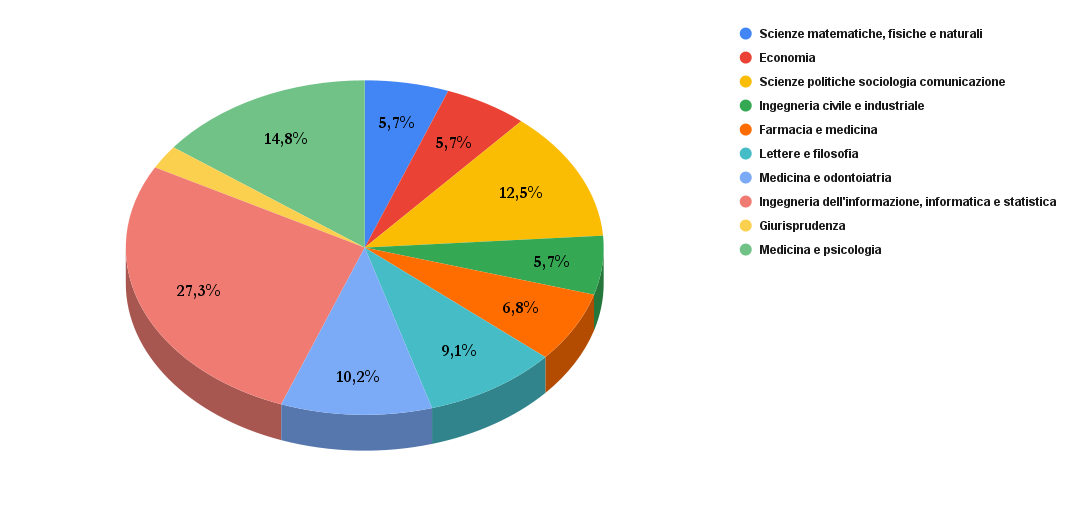
\includegraphics[width=1.1\textwidth]{/Users/leonardvincentramil/Desktop/MyDoc/MyLatex/ProgettoINTRUSIACSAI/01_NeedFinding/img/01.png}
    \end{center}    

    \item Triennale o Magistrale?
    \begin{center}
        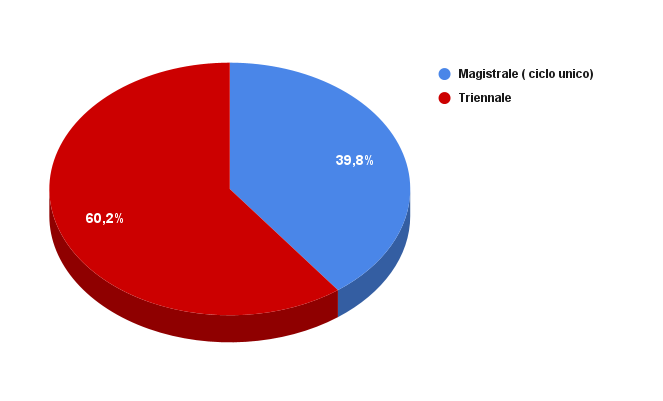
\includegraphics[width=0.65\textwidth]{/Users/leonardvincentramil/Desktop/MyDoc/MyLatex/ProgettoINTRUSIACSAI/01_NeedFinding/img/02.png}
    \end{center}
    \item Sai se nel tuo corso di laurea sono presenti corsi a scelta?
    \begin{center}
        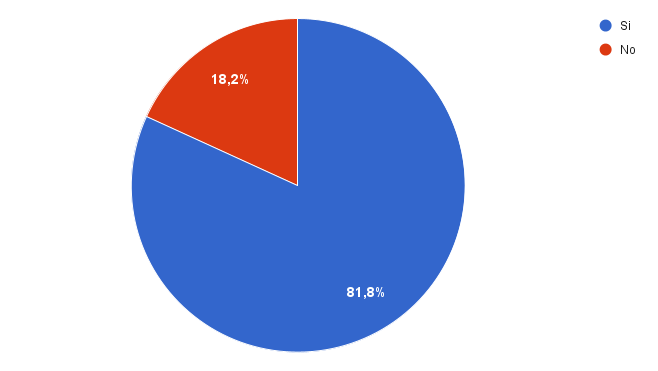
\includegraphics[width=0.7\textwidth]{/Users/leonardvincentramil/Desktop/MyDoc/MyLatex/ProgettoINTRUSIACSAI/01_NeedFinding/img/03.png}
    \end{center}   
    \begin{enumerate}
        \item SI (Branch: Continua con le domande Corsi a Scelta)
        \item NO (Branch: Continua con le domande sulle Opinioni riguardo i Professori)
    \end{enumerate}
\end{enumerate}

\subsubsection{Domande Corsi a Scelta (Percorso Formativo)}
\begin{enumerate}
    \item (Come hai reperito/ricercato i corsi?) Come hai scelto i corsi?
    \begin{center}
        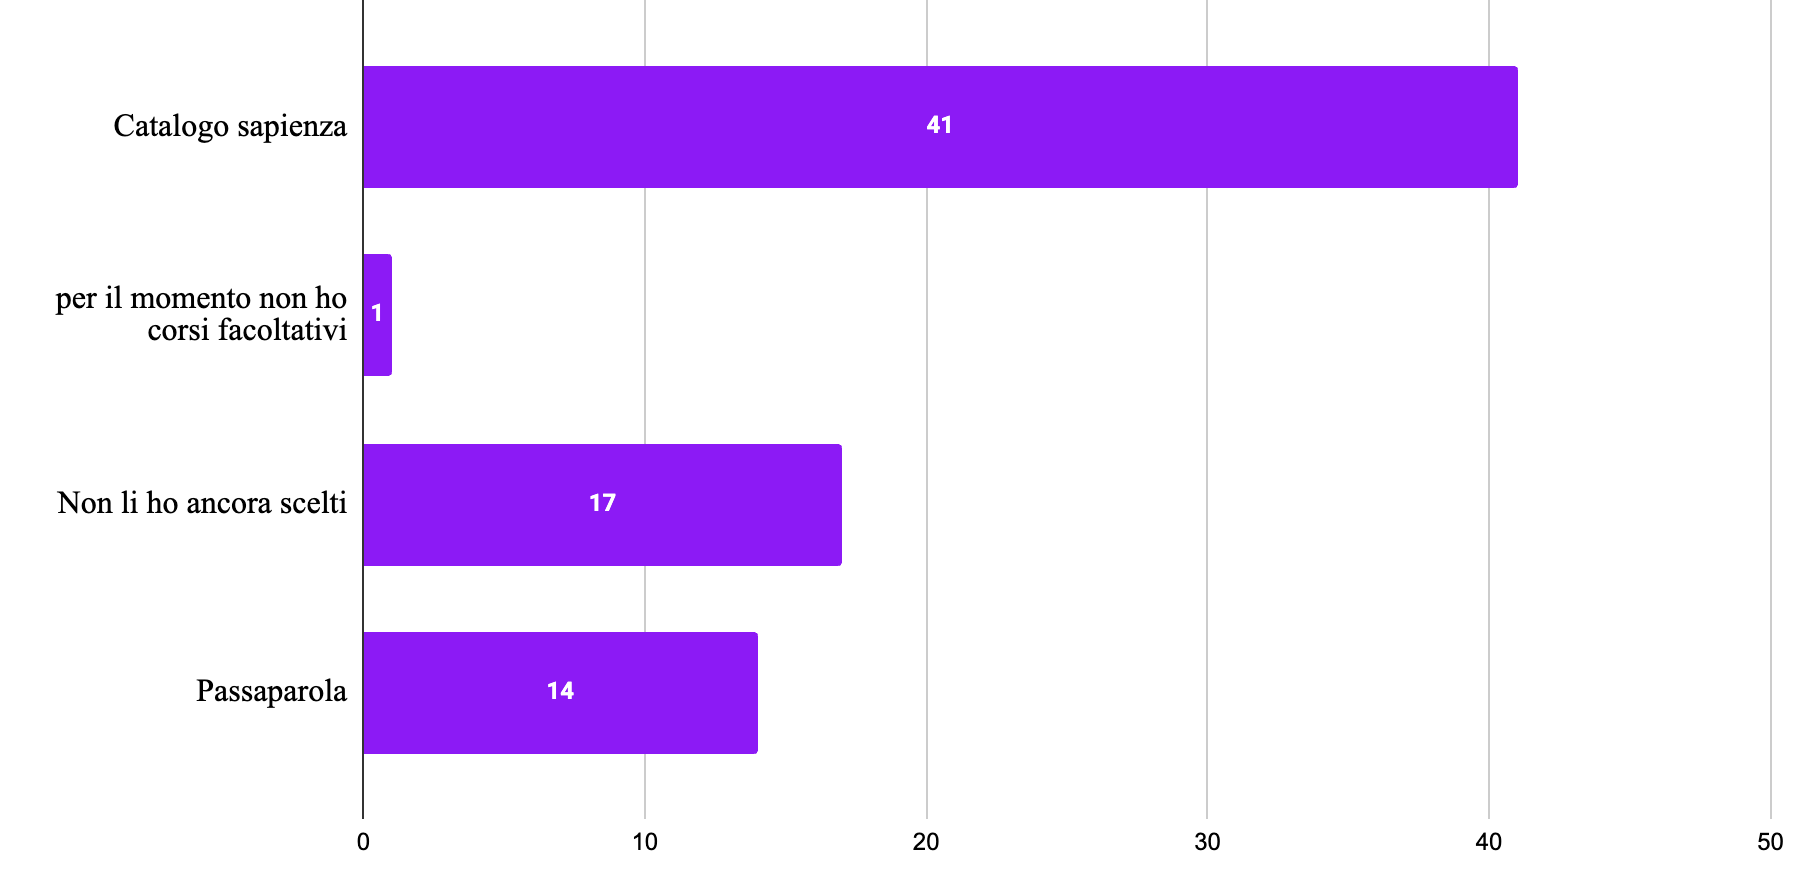
\includegraphics[width=0.9\textwidth]{/Users/leonardvincentramil/Desktop/MyDoc/MyLatex/ProgettoINTRUSIACSAI/01_NeedFinding/img/04.png}
    \end{center} 
    \item Quali dei seguenti aspetti riguardanti la compilazione del percorso formativo è risultato poco chiaro? (più scelta)
    \begin{center}
        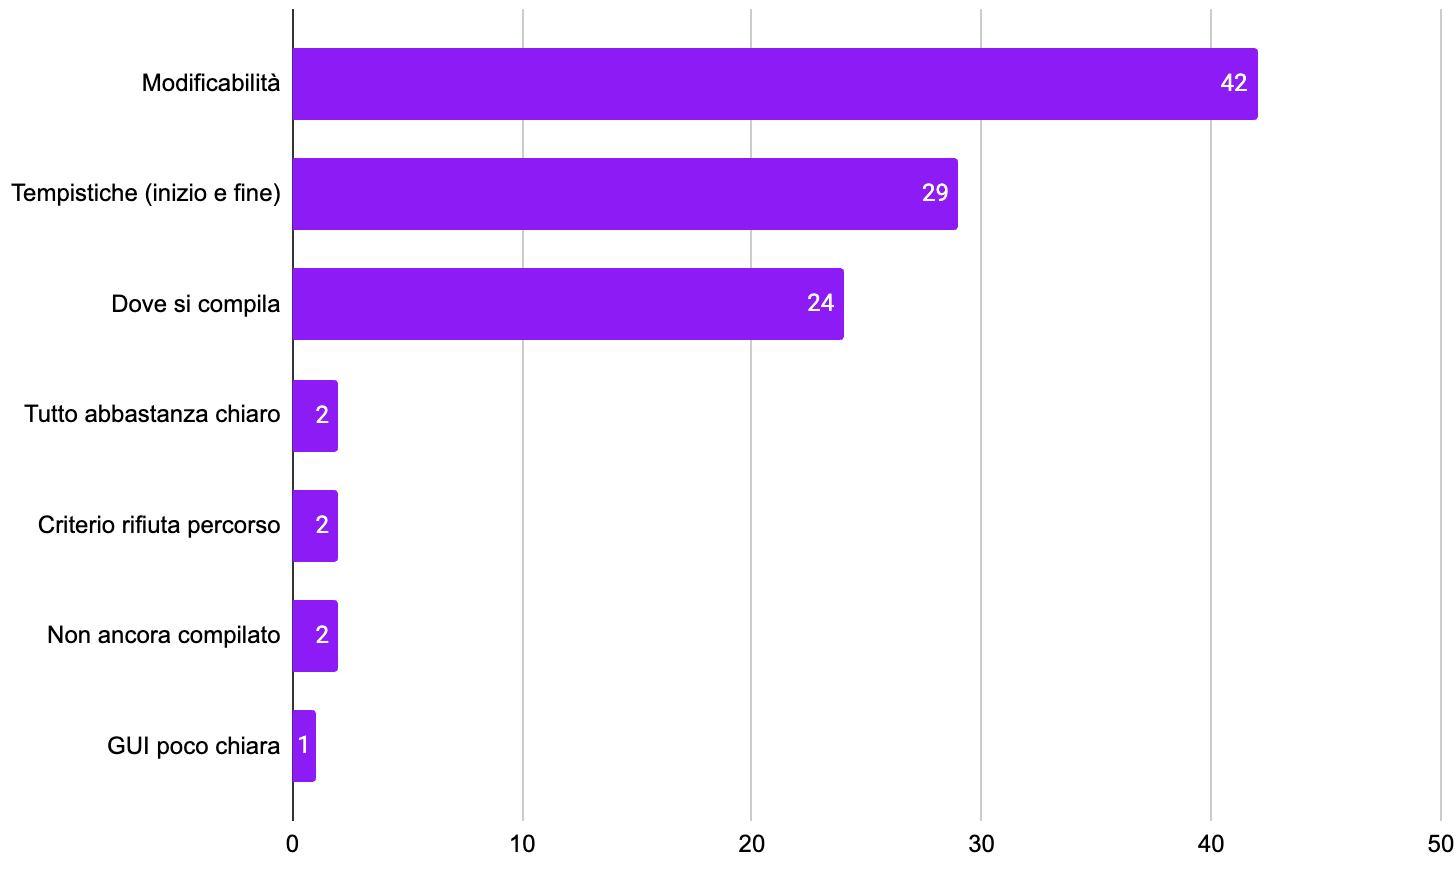
\includegraphics[width=0.85\textwidth]{/Users/leonardvincentramil/Desktop/MyDoc/MyLatex/ProgettoINTRUSIACSAI/01_NeedFinding/img/05.png}
    \end{center}
    \item Quanto la scelta del percorso formativo dipende da quello in cui ti vuoi specializzare?
    \begin{center}
        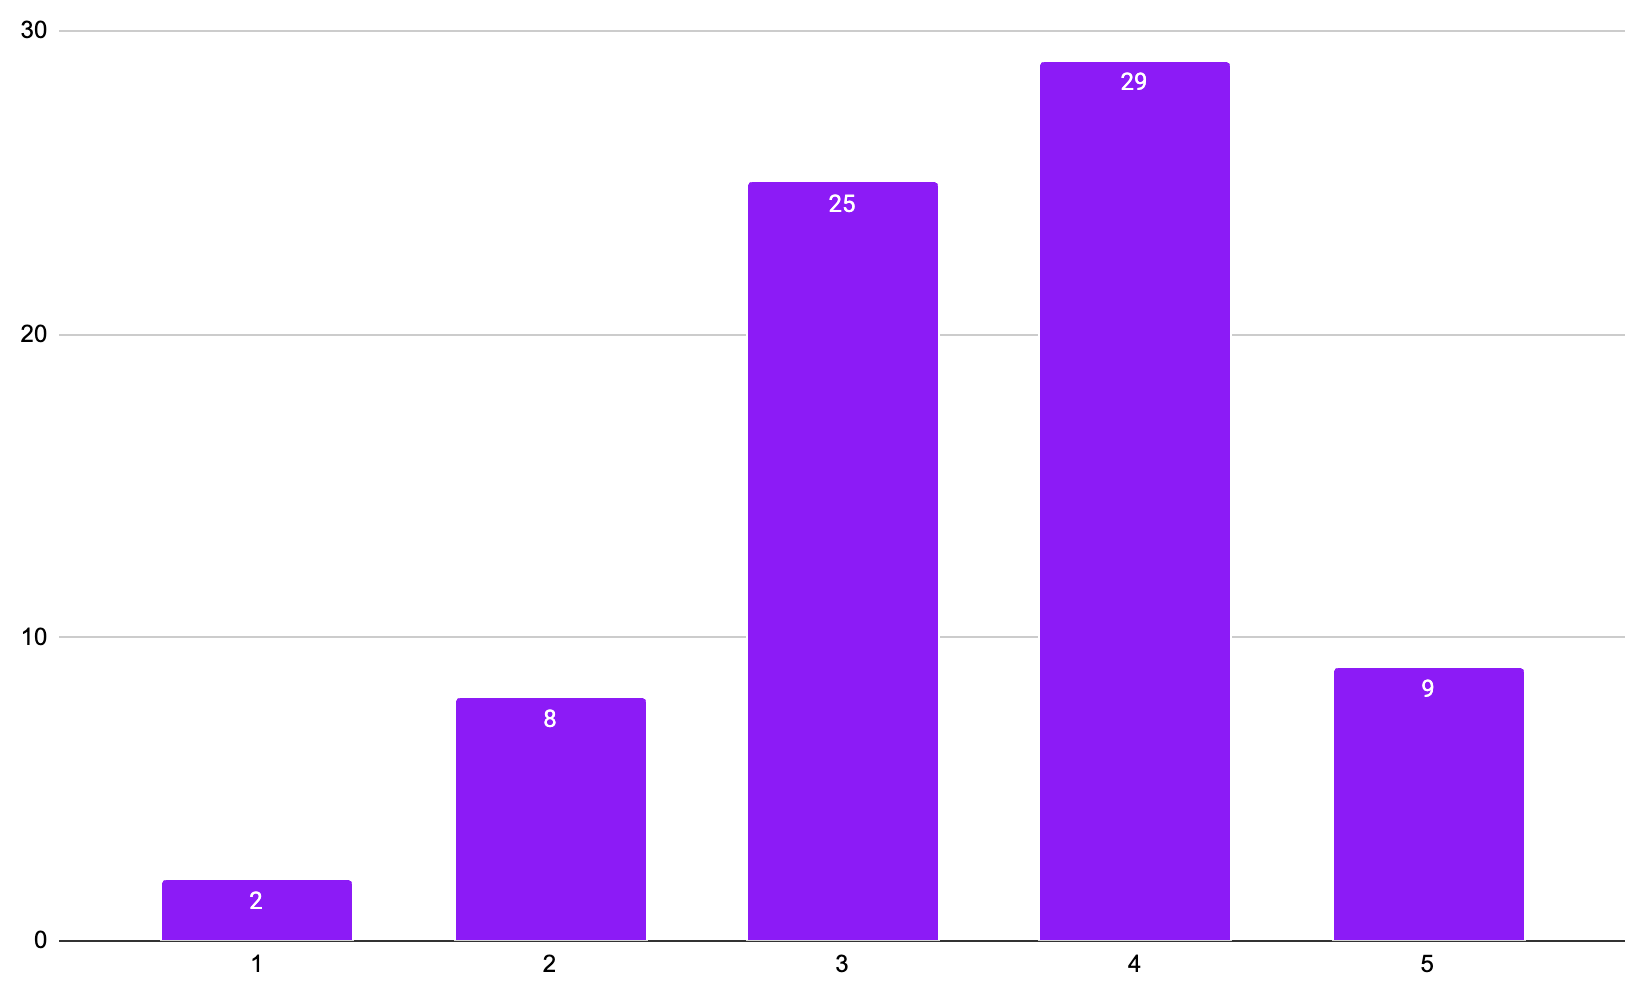
\includegraphics[width=0.8\textwidth]{/Users/leonardvincentramil/Desktop/MyDoc/MyLatex/ProgettoINTRUSIACSAI/01_NeedFinding/img/06.png}
    \end{center} 
    \item Seleziona tra le seguenti una o più situazioni in cui ti sei trovato:
    \begin{center}
        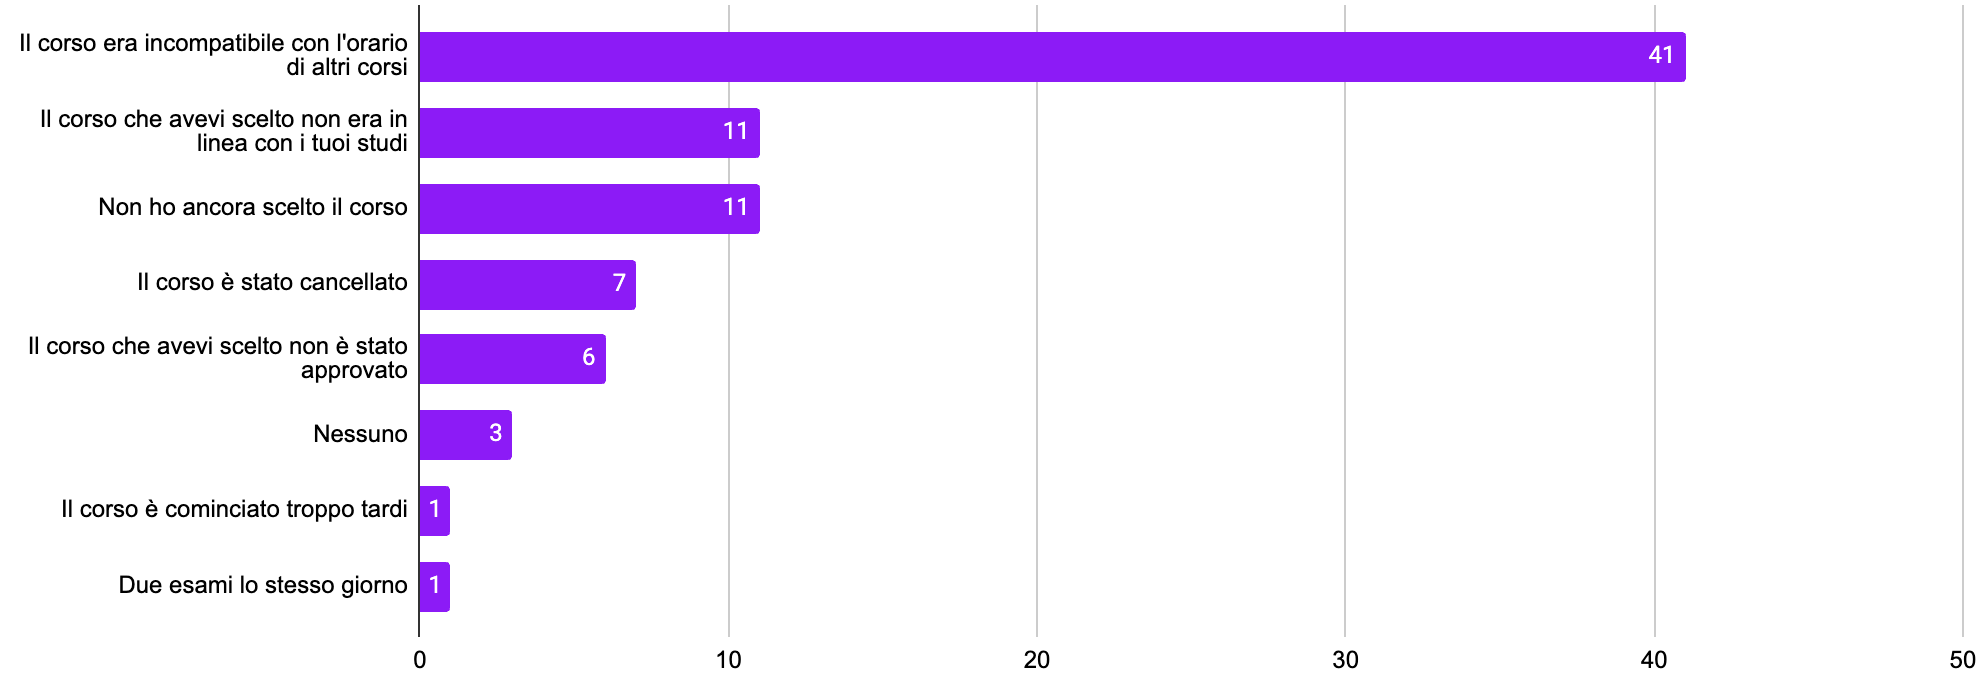
\includegraphics[width=1.0\textwidth]{/Users/leonardvincentramil/Desktop/MyDoc/MyLatex/ProgettoINTRUSIACSAI/01_NeedFinding/img/07.png}
    \end{center}
    \item Nella scelta quanto influisce il professore del corso:
    \begin{center}
        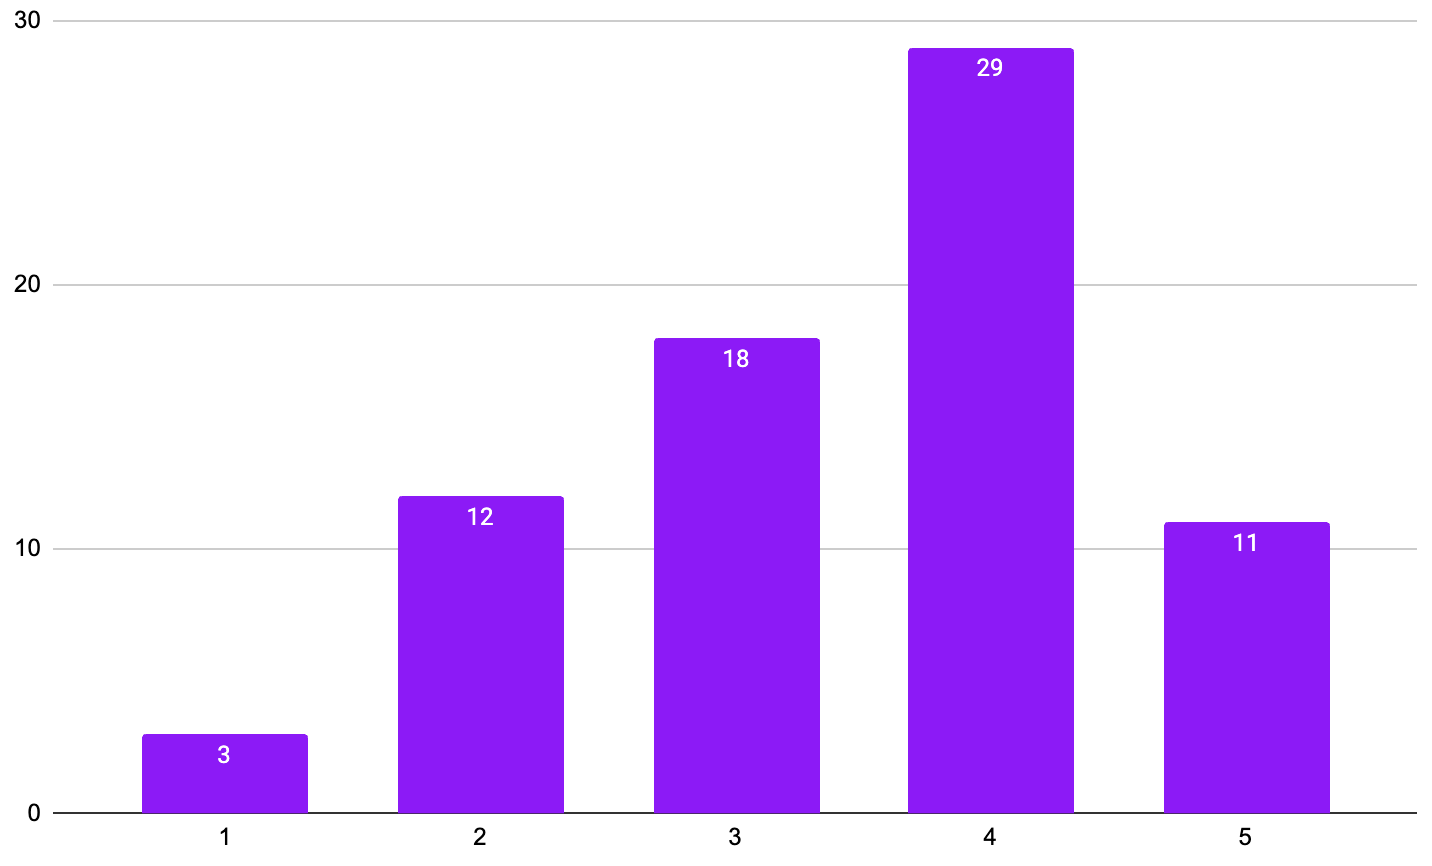
\includegraphics[width=0.75\textwidth]{/Users/leonardvincentramil/Desktop/MyDoc/MyLatex/ProgettoINTRUSIACSAI/01_NeedFinding/img/08.png}
    \end{center} 
    \item Nella scelta quanto influsice la modalità di esame (orale, progetto):
    \begin{center}
        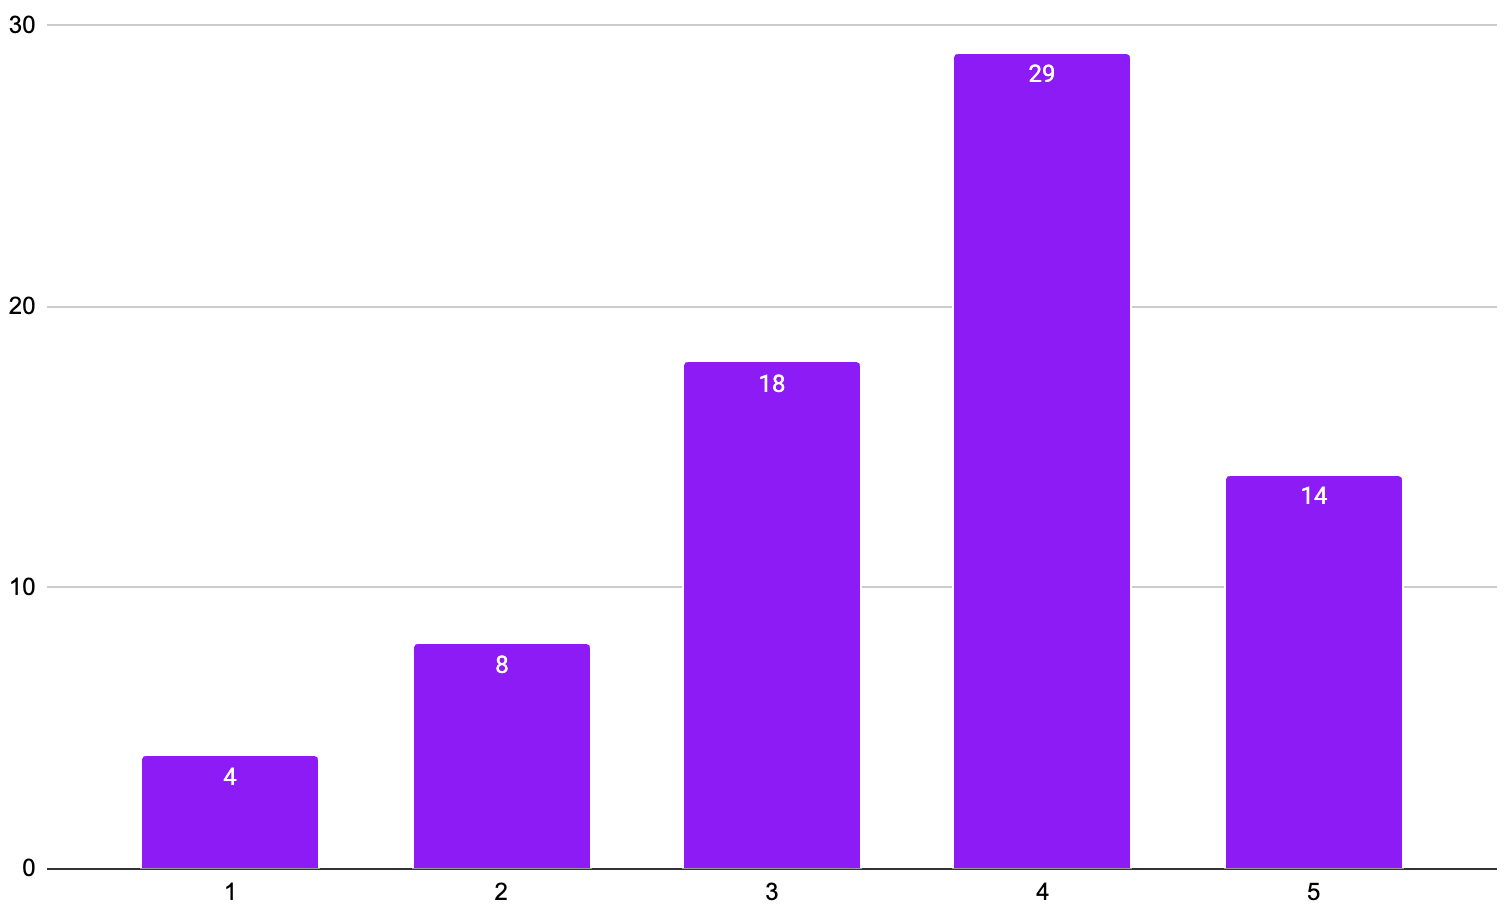
\includegraphics[width=0.75\textwidth]{/Users/leonardvincentramil/Desktop/MyDoc/MyLatex/ProgettoINTRUSIACSAI/01_NeedFinding/img/09.png}
    \end{center} 
\end{enumerate}

\subsubsection{Domande sulle Opinioni riguardo i Professori}
\begin{enumerate}
    \item Generalmente nel tuo percorso di studi quanto ti interessa del professore che terrà il corso?
    \begin{center}
        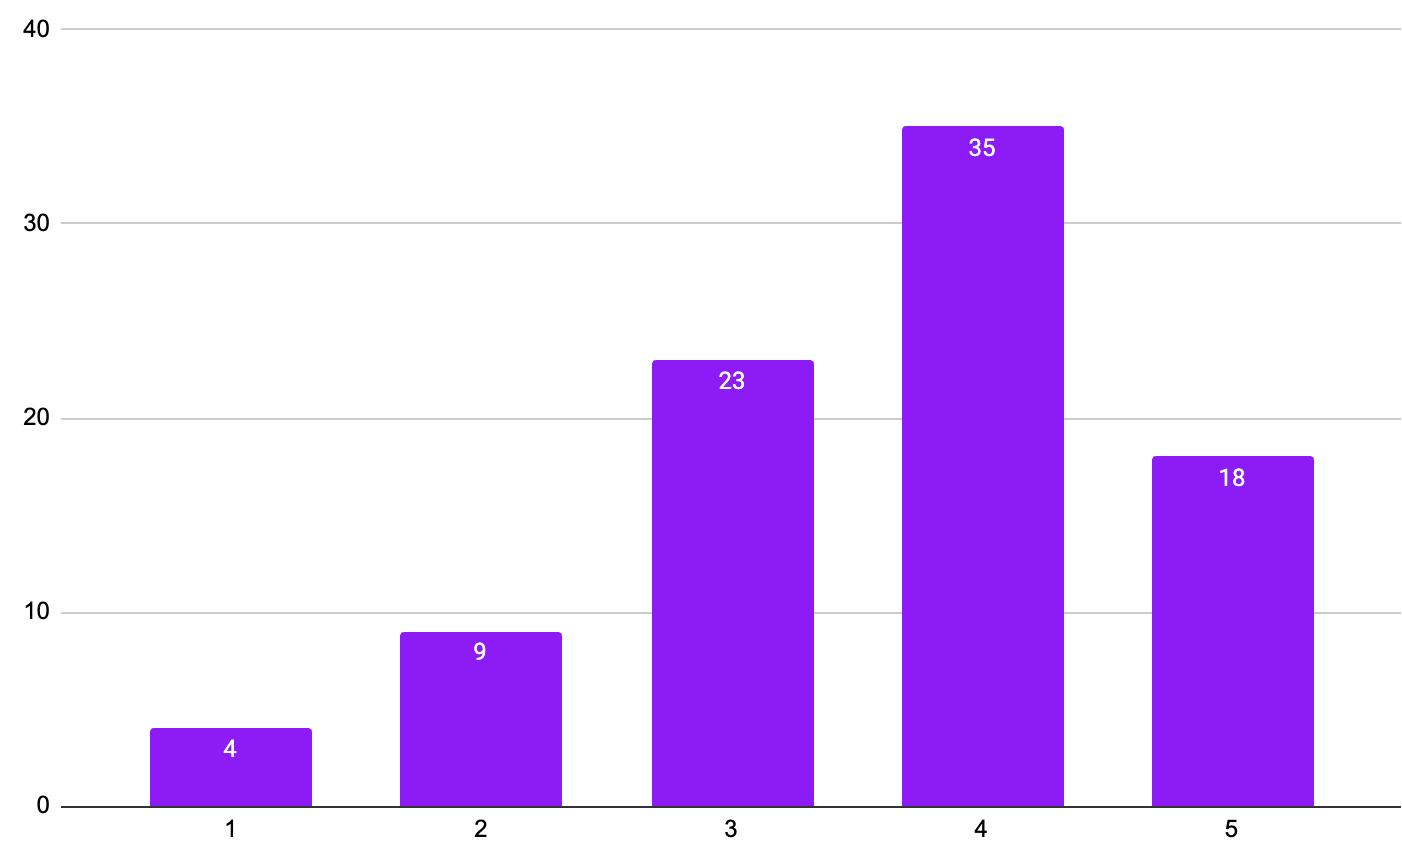
\includegraphics[width=0.7\textwidth]{/Users/leonardvincentramil/Desktop/MyDoc/MyLatex/ProgettoINTRUSIACSAI/01_NeedFinding/img/10.png}
    \end{center}     

    \item Quanto ti interessa l'opinione degli studenti riguardo i professori?
    \begin{center}
        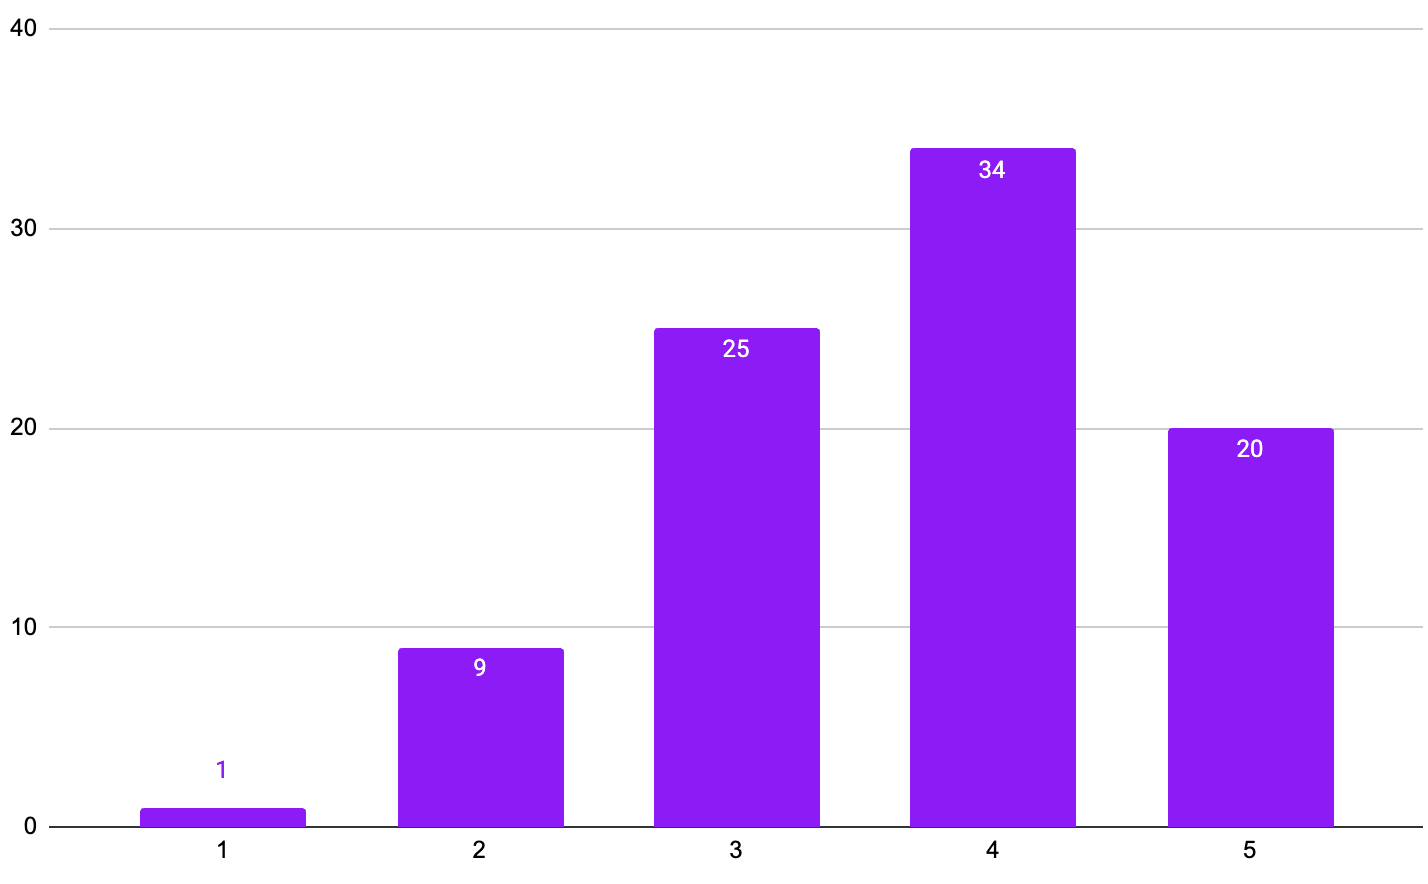
\includegraphics[width=0.8\textwidth]{/Users/leonardvincentramil/Desktop/MyDoc/MyLatex/ProgettoINTRUSIACSAI/01_NeedFinding/img/11.png}
    \end{center} 
    \item Quali informazioni ti interessano nella ricerca del professore:
    \begin{center}
        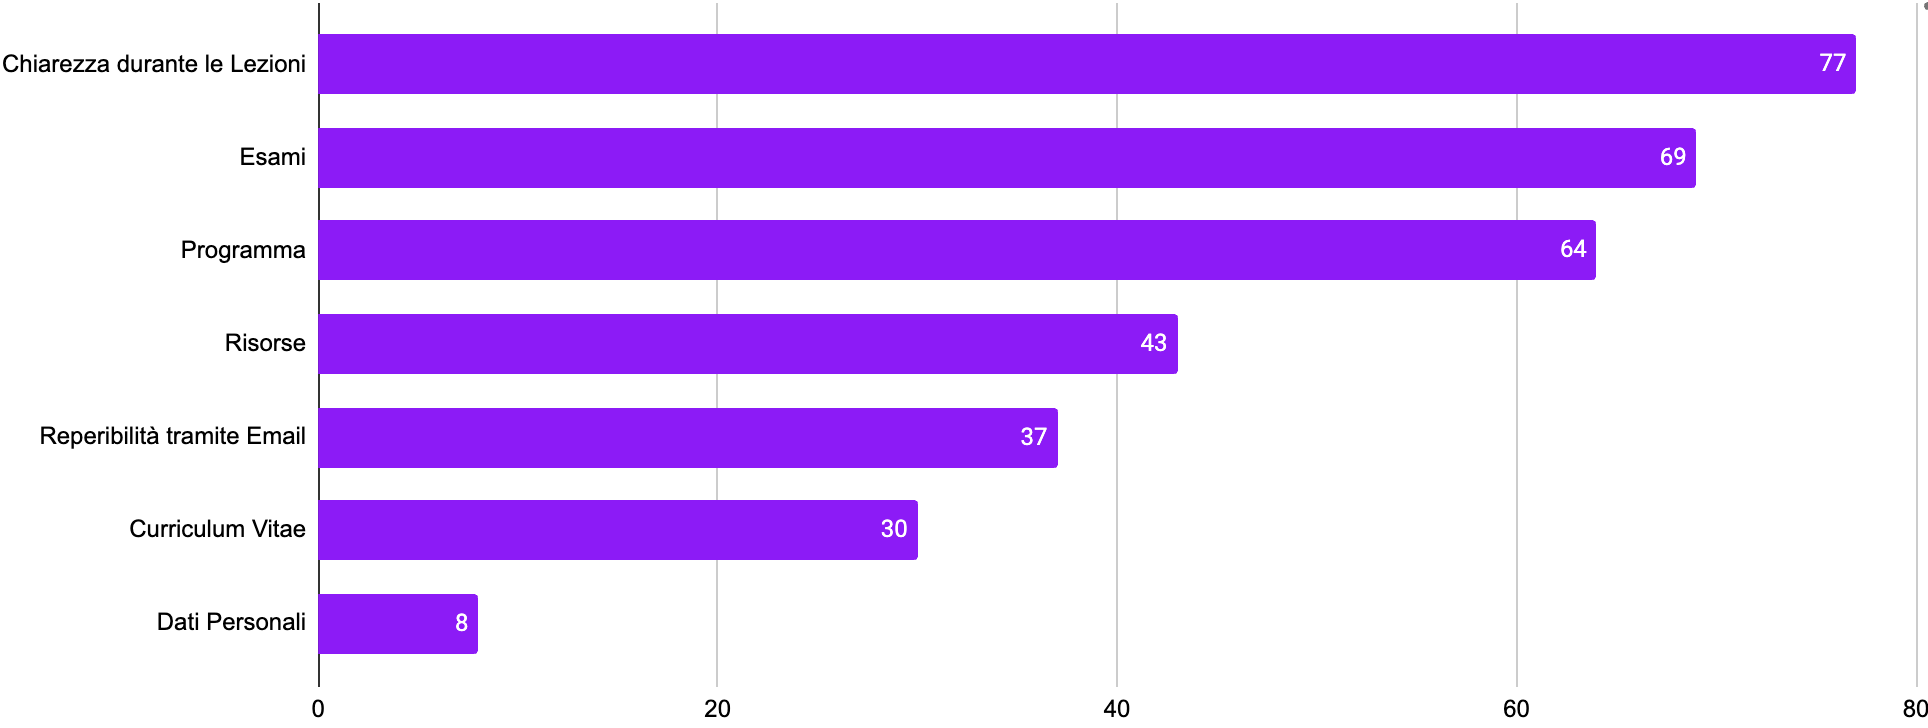
\includegraphics[width=1.1\textwidth]{/Users/leonardvincentramil/Desktop/MyDoc/MyLatex/ProgettoINTRUSIACSAI/01_NeedFinding/img/12.png}
    \end{center}
    \item Ti è semplice reperire il materiale del professore (sia quello utilizzato a lezione ch quello al di fuori: libri, articoli)
    \begin{center}
        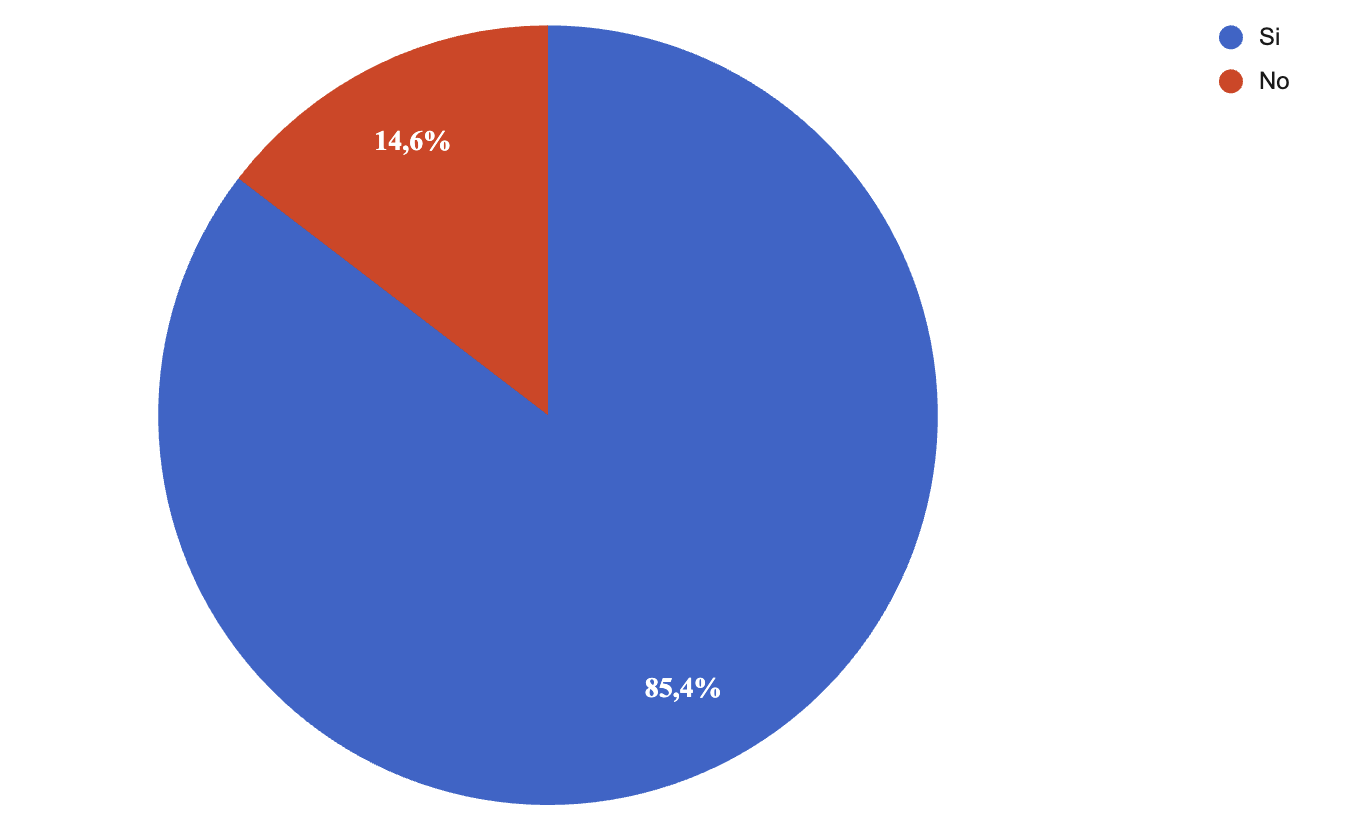
\includegraphics[width=0.7\textwidth]{/Users/leonardvincentramil/Desktop/MyDoc/MyLatex/ProgettoINTRUSIACSAI/01_NeedFinding/img/13.png}
    \end{center} 
    \item Quanto la disponibilità della condivisione dei materiali dai tuoi colleghi ti può essere utile?
    \begin{center}
        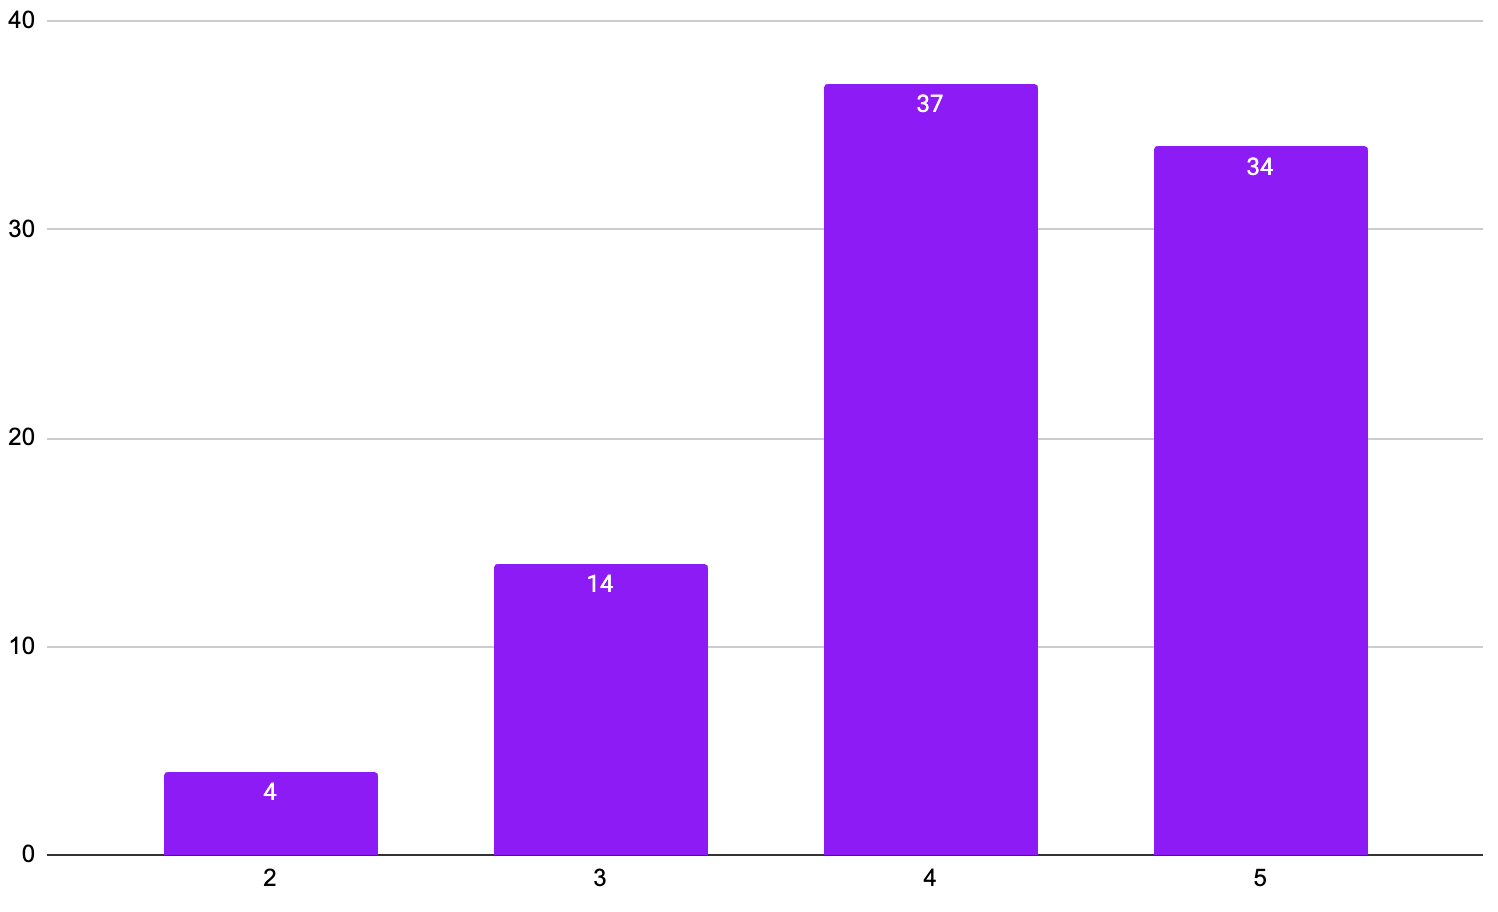
\includegraphics[width=0.8\textwidth]{/Users/leonardvincentramil/Desktop/MyDoc/MyLatex/ProgettoINTRUSIACSAI/01_NeedFinding/img/14.png}
    \end{center} 
    \item Nel tuo Corso di Laurea è previsto un tirocinio?
    \begin{center}
        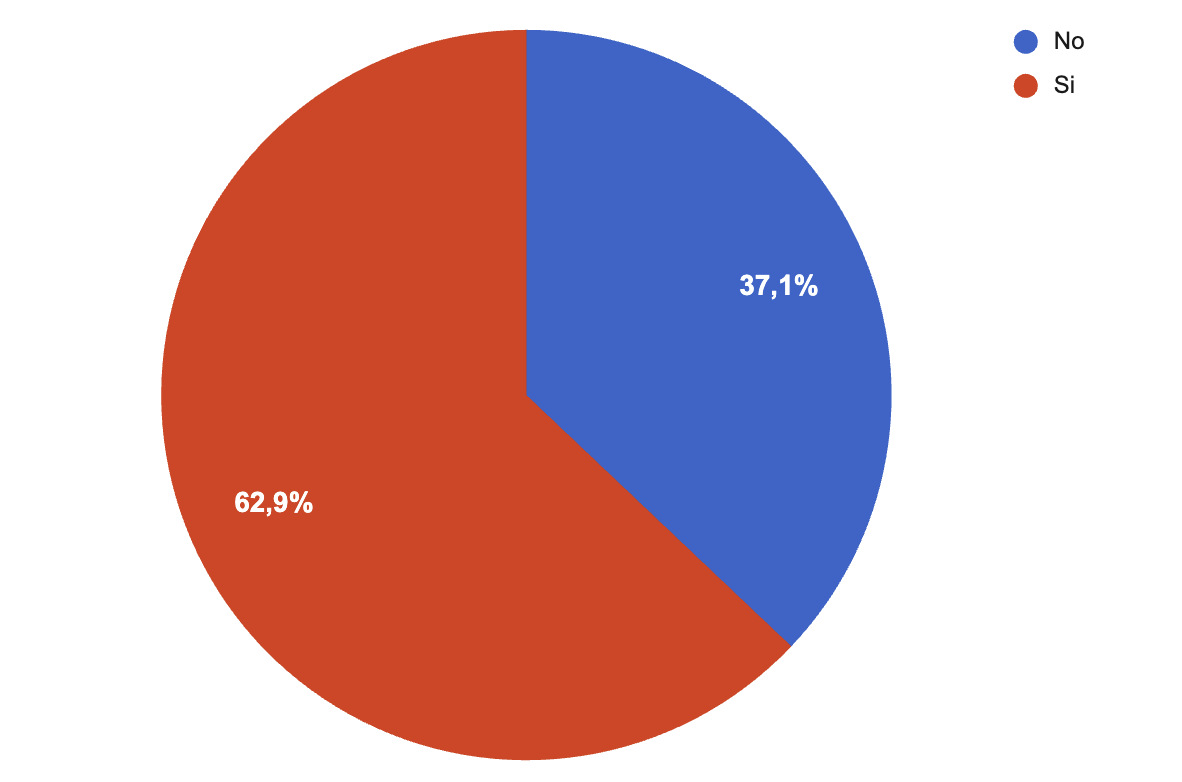
\includegraphics[width=0.6\textwidth]{/Users/leonardvincentramil/Desktop/MyDoc/MyLatex/ProgettoINTRUSIACSAI/01_NeedFinding/img/15.png}
    \end{center} 
    \begin{enumerate}
        \item SI (Branch: Continua con le domande sul Tirocinio)
        \item NO (Questionario Finito)
    \end{enumerate}
\end{enumerate}

\subsubsection{Domande sul Tirocinio}
\begin{enumerate}
    \item Quali dei seguenti aspetti riguardanti la compilazione del tirocinio risultano poco chiari:
    \begin{center}
        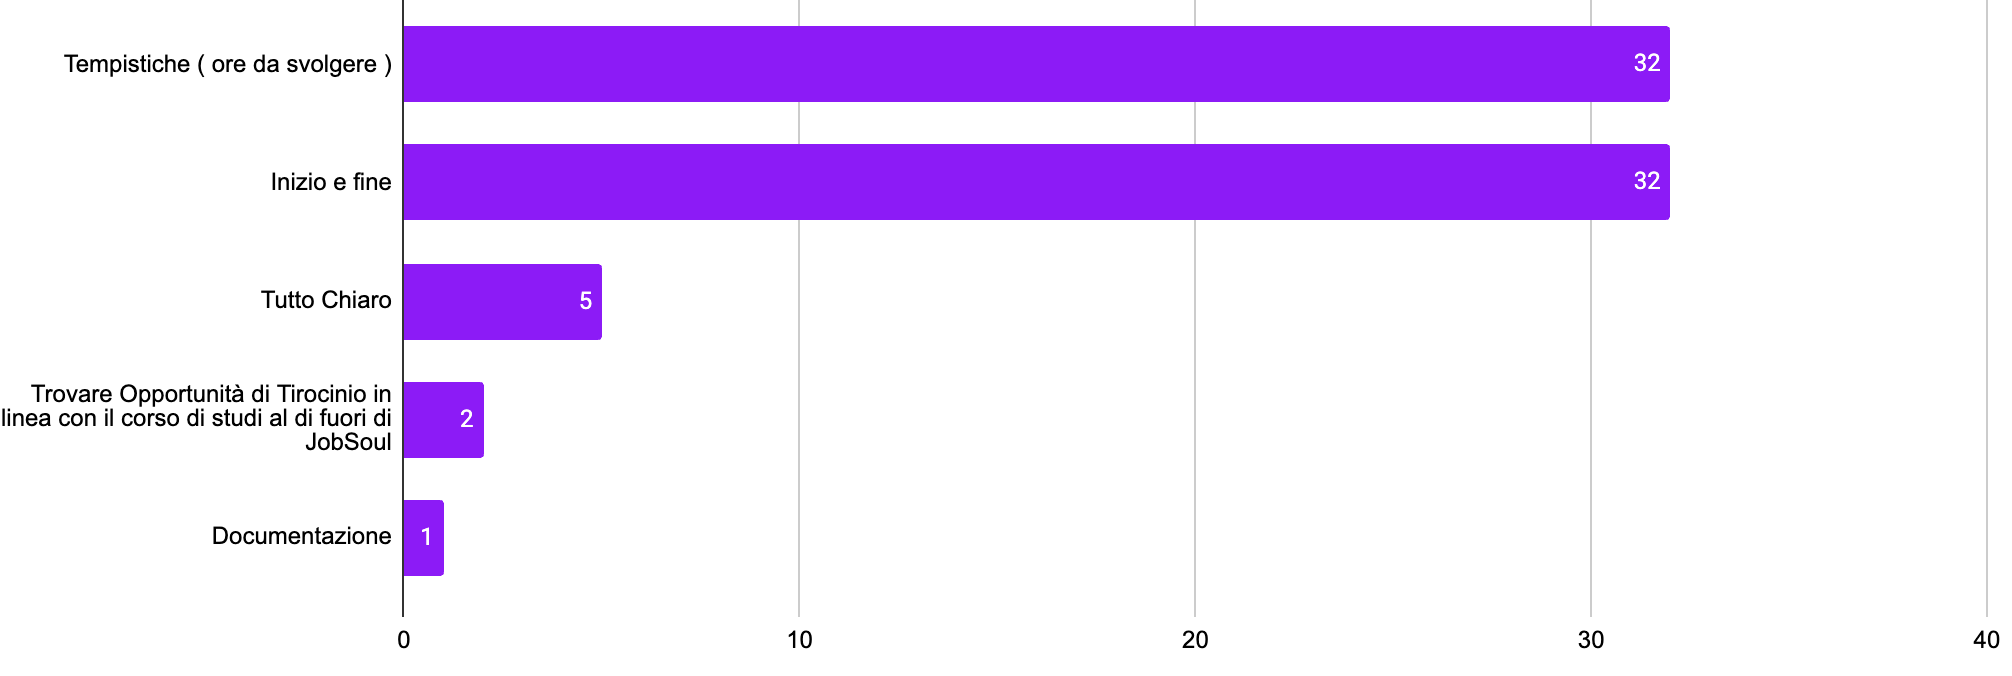
\includegraphics[width=1.0\textwidth]{/Users/leonardvincentramil/Desktop/MyDoc/MyLatex/ProgettoINTRUSIACSAI/01_NeedFinding/img/16.png}
    \end{center}
    \item Pensi di farlo o lo hai già fatto Interno o Esterno?
    \begin{center}
        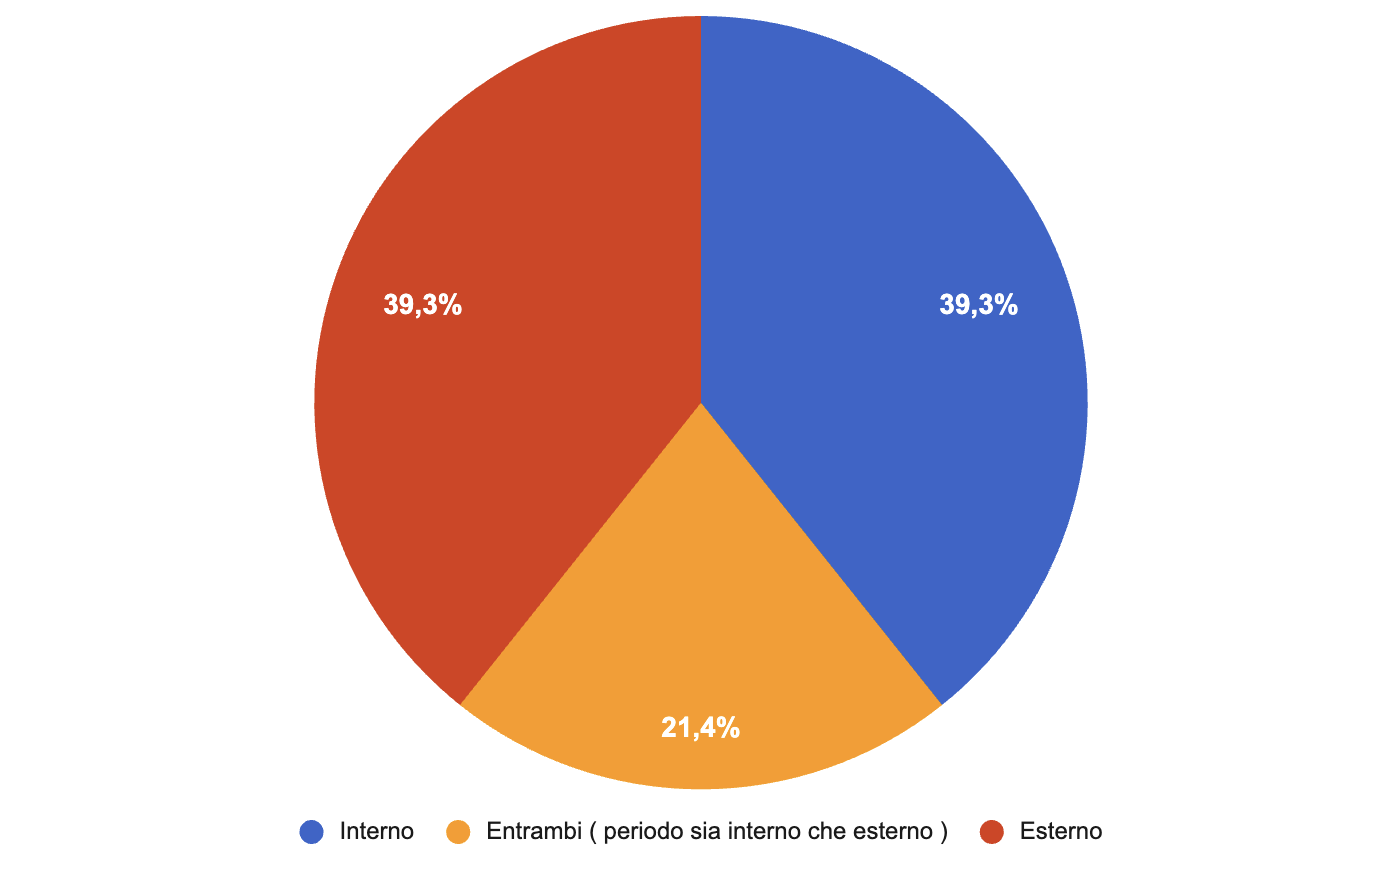
\includegraphics[width=0.8\textwidth]{/Users/leonardvincentramil/Desktop/MyDoc/MyLatex/ProgettoINTRUSIACSAI/01_NeedFinding/img/17.png}
    \end{center} 
    \begin{enumerate}
        \item Esterno (Questionario Finito)
        \item Interno (Branch: Continua con le domande sul Tirocinio Interno)
        \item Entrambi (Periodo sia Interno che Esterno) (Branch: Continua con le domande sul Tirocinio Interno)
    \end{enumerate}
    \textbf{Domande Tirocinio Interno}
    \item Considerando solo il tirocinio interno, le informazoni a riguardo come ti sono sembrate?
    \begin{center}
        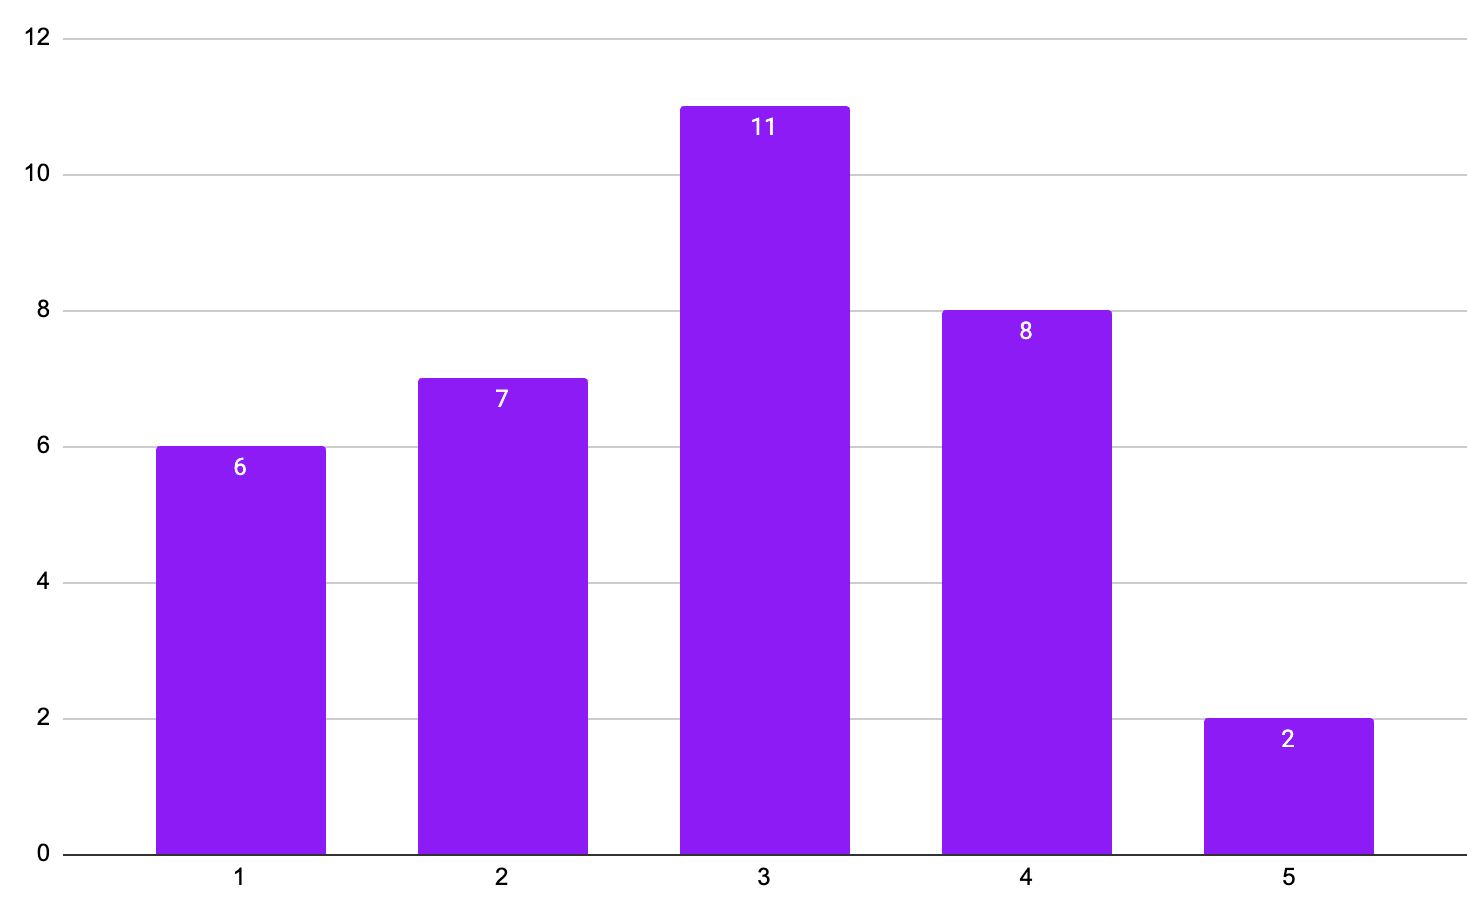
\includegraphics[width=1.0\textwidth]{/Users/leonardvincentramil/Desktop/MyDoc/MyLatex/ProgettoINTRUSIACSAI/01_NeedFinding/img/18.png}
    \end{center} 
    \item Considerando solo il tirocinio interno, la scelta del professore è stata indotta o sarà indotta da te o da sapienza?
    \begin{center}
        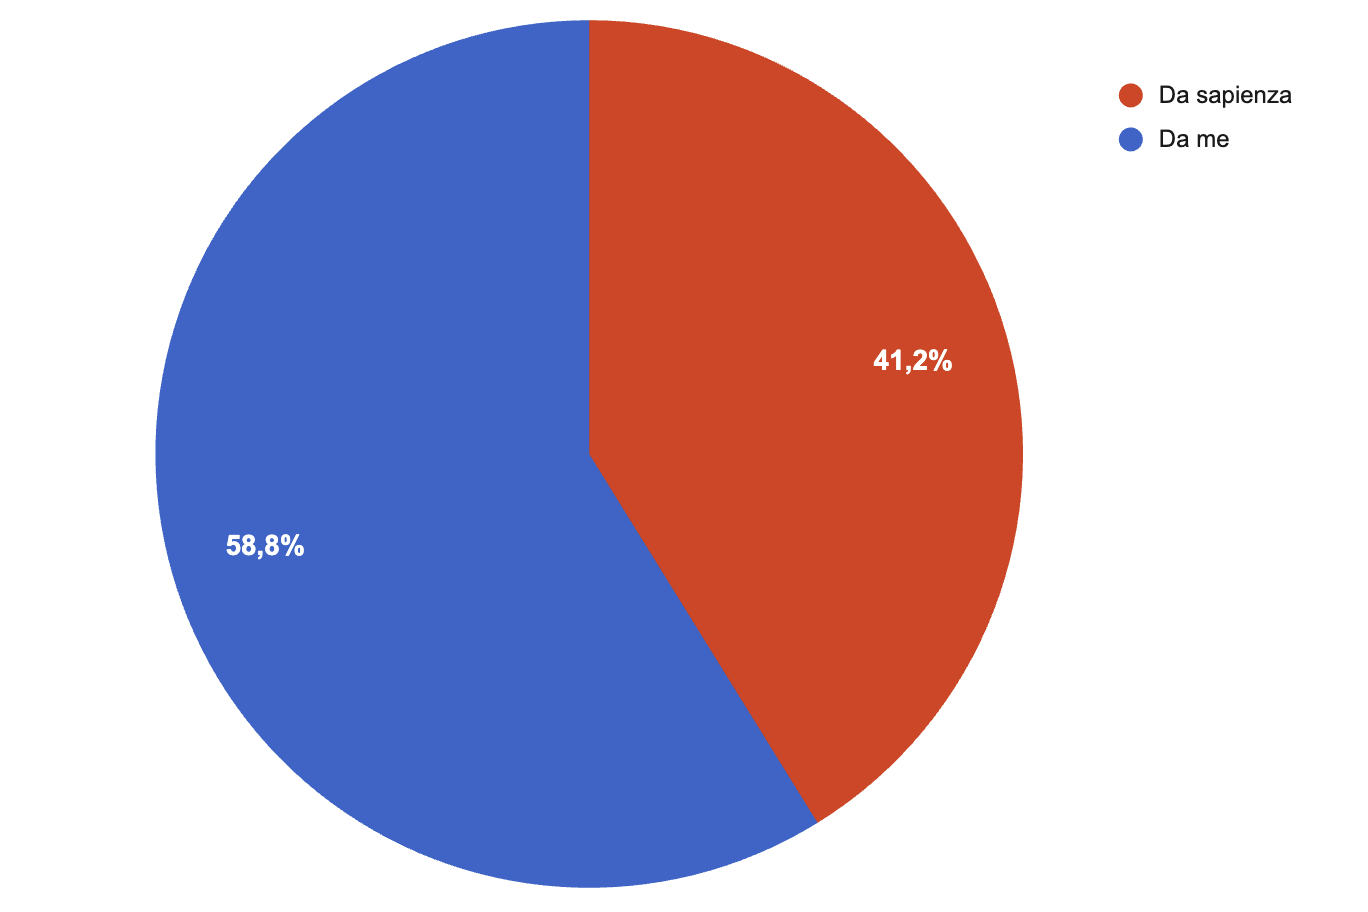
\includegraphics[width=0.65\textwidth]{/Users/leonardvincentramil/Desktop/MyDoc/MyLatex/ProgettoINTRUSIACSAI/01_NeedFinding/img/19.png}
    \end{center} 
    \begin{enumerate}
        \item Da me (Branch: Continua con le domande sul Tirocinio Scelto da Me)
        \item Da Sapienza (Branch: Continua con le domande sul Tirocinio Scelto da Sapienza)
    \end{enumerate}
\end{enumerate}

\textbf{Sezione: domande sul Tirocinio Scelto da Sapienza}
\begin{enumerate}
    \item Anche se la scelta è stata o sarà indotta da sapienza, ti sei comunque interessato o pensi ti interesserai al professore che ti avrebbe seguito nel percorso di tirocinio ?
    \begin{center}
        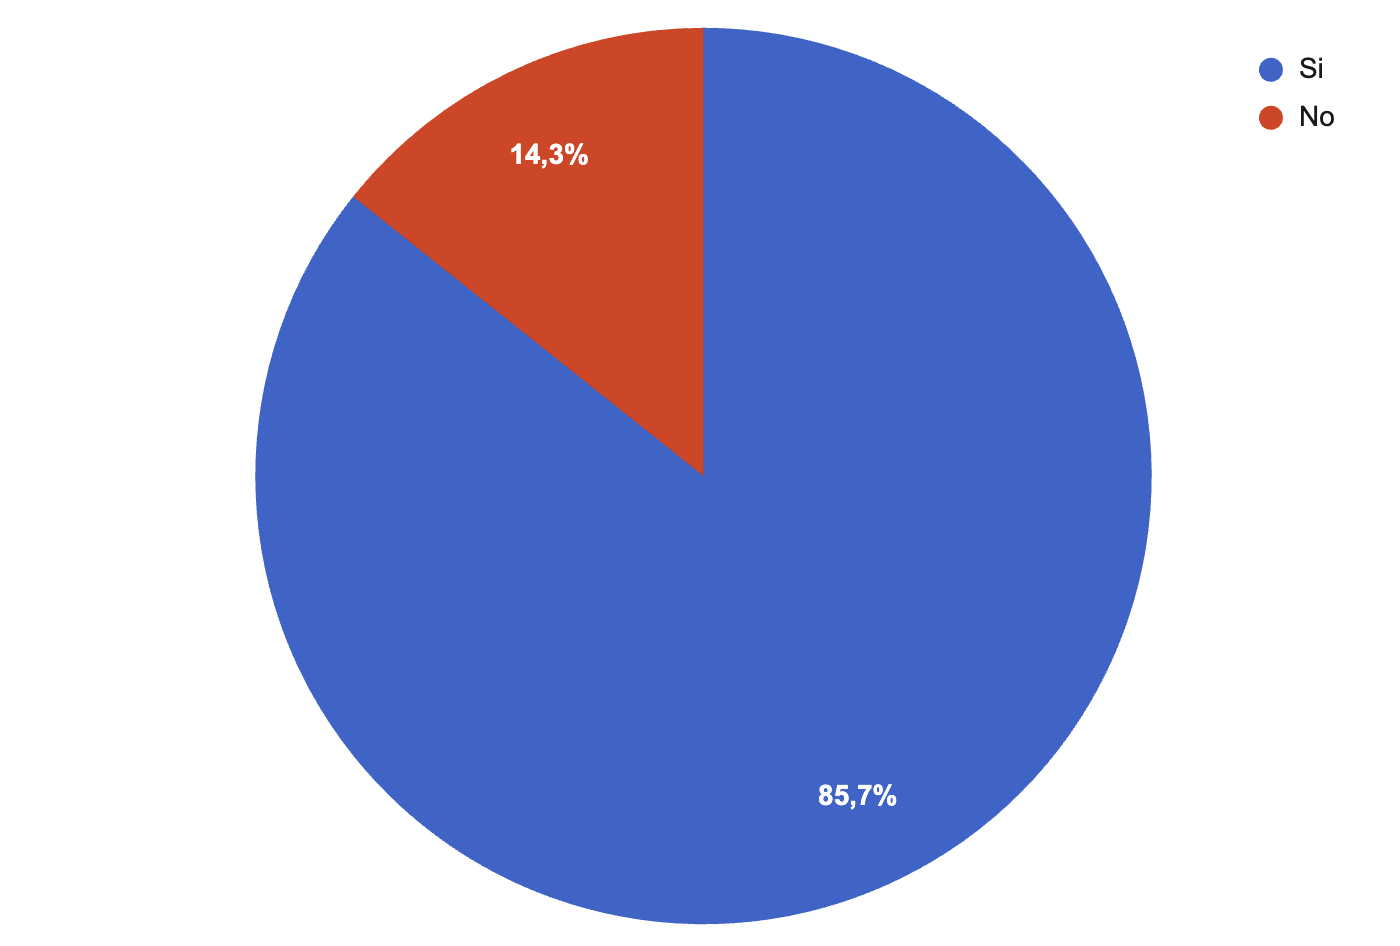
\includegraphics[width=0.65\textwidth]{/Users/leonardvincentramil/Desktop/MyDoc/MyLatex/ProgettoINTRUSIACSAI/01_NeedFinding/img/20.png}
    \end{center} 
    \item Quale di queste fonti hai utilizzato (o pensi di utilizzare) per conoscere meglio il tuo professore:
    \begin{center}
        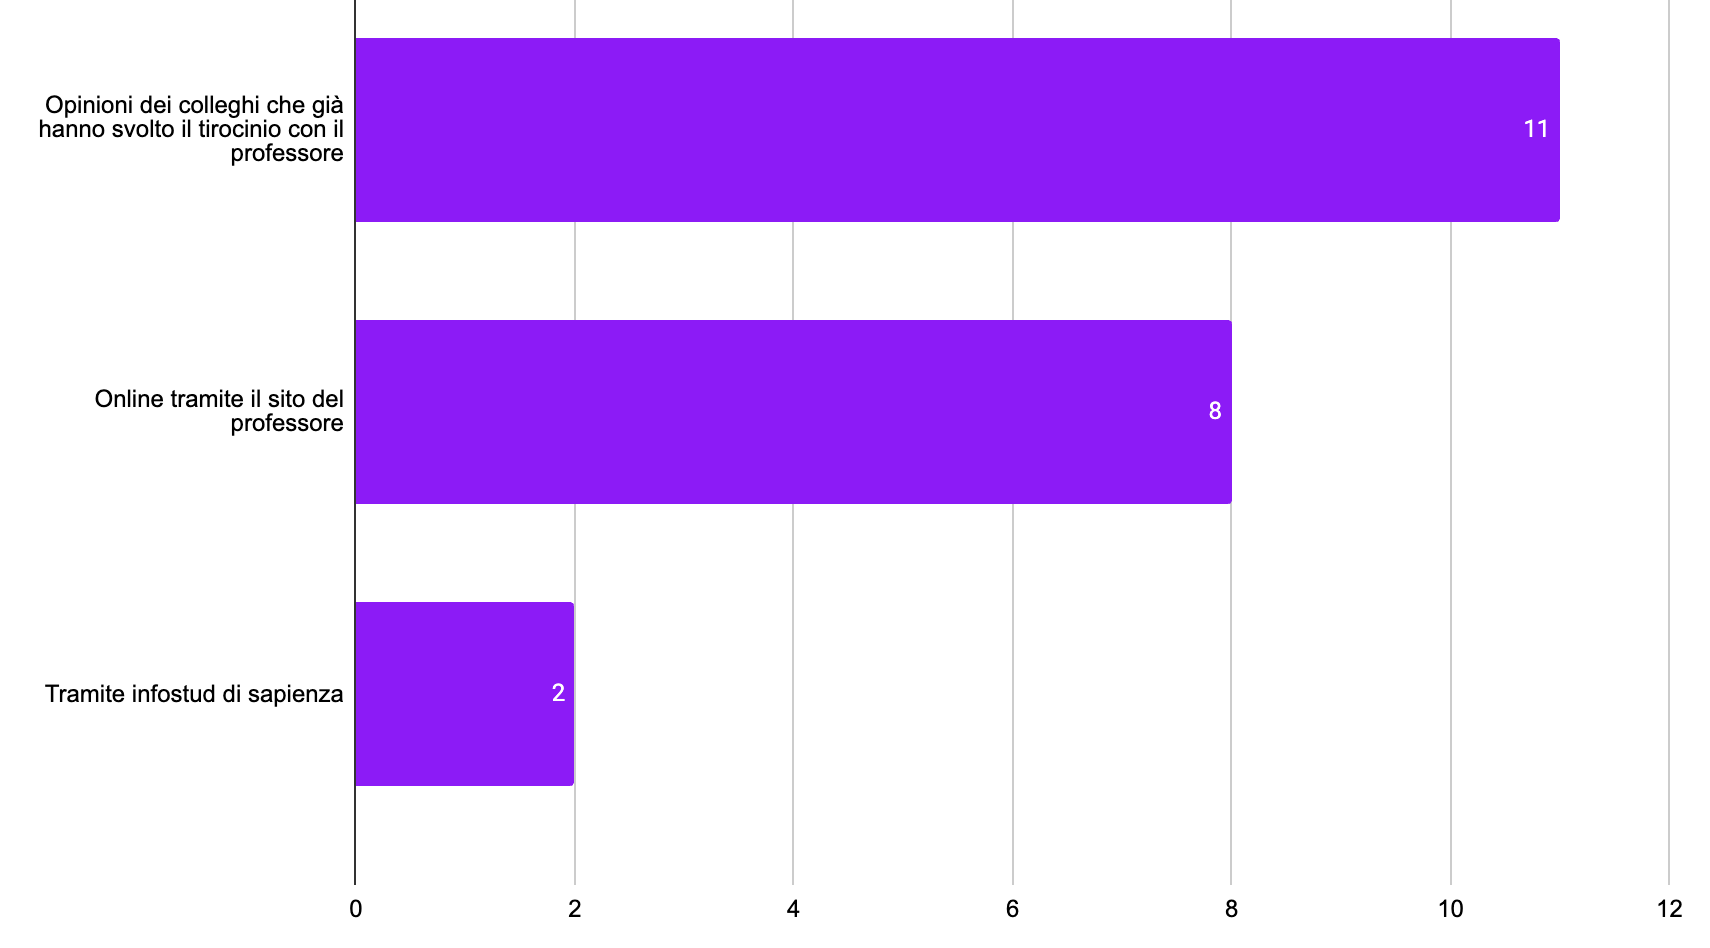
\includegraphics[width=0.75\textwidth]{/Users/leonardvincentramil/Desktop/MyDoc/MyLatex/ProgettoINTRUSIACSAI/01_NeedFinding/img/21.png}
    \end{center}
\end{enumerate}

\textbf{Sezione: domande sul Tirocinio Scelto da Me}
\begin{enumerate}
    \item Se utilizzi dei criteri per scegliee il professore quali sono:
    \begin{center}
        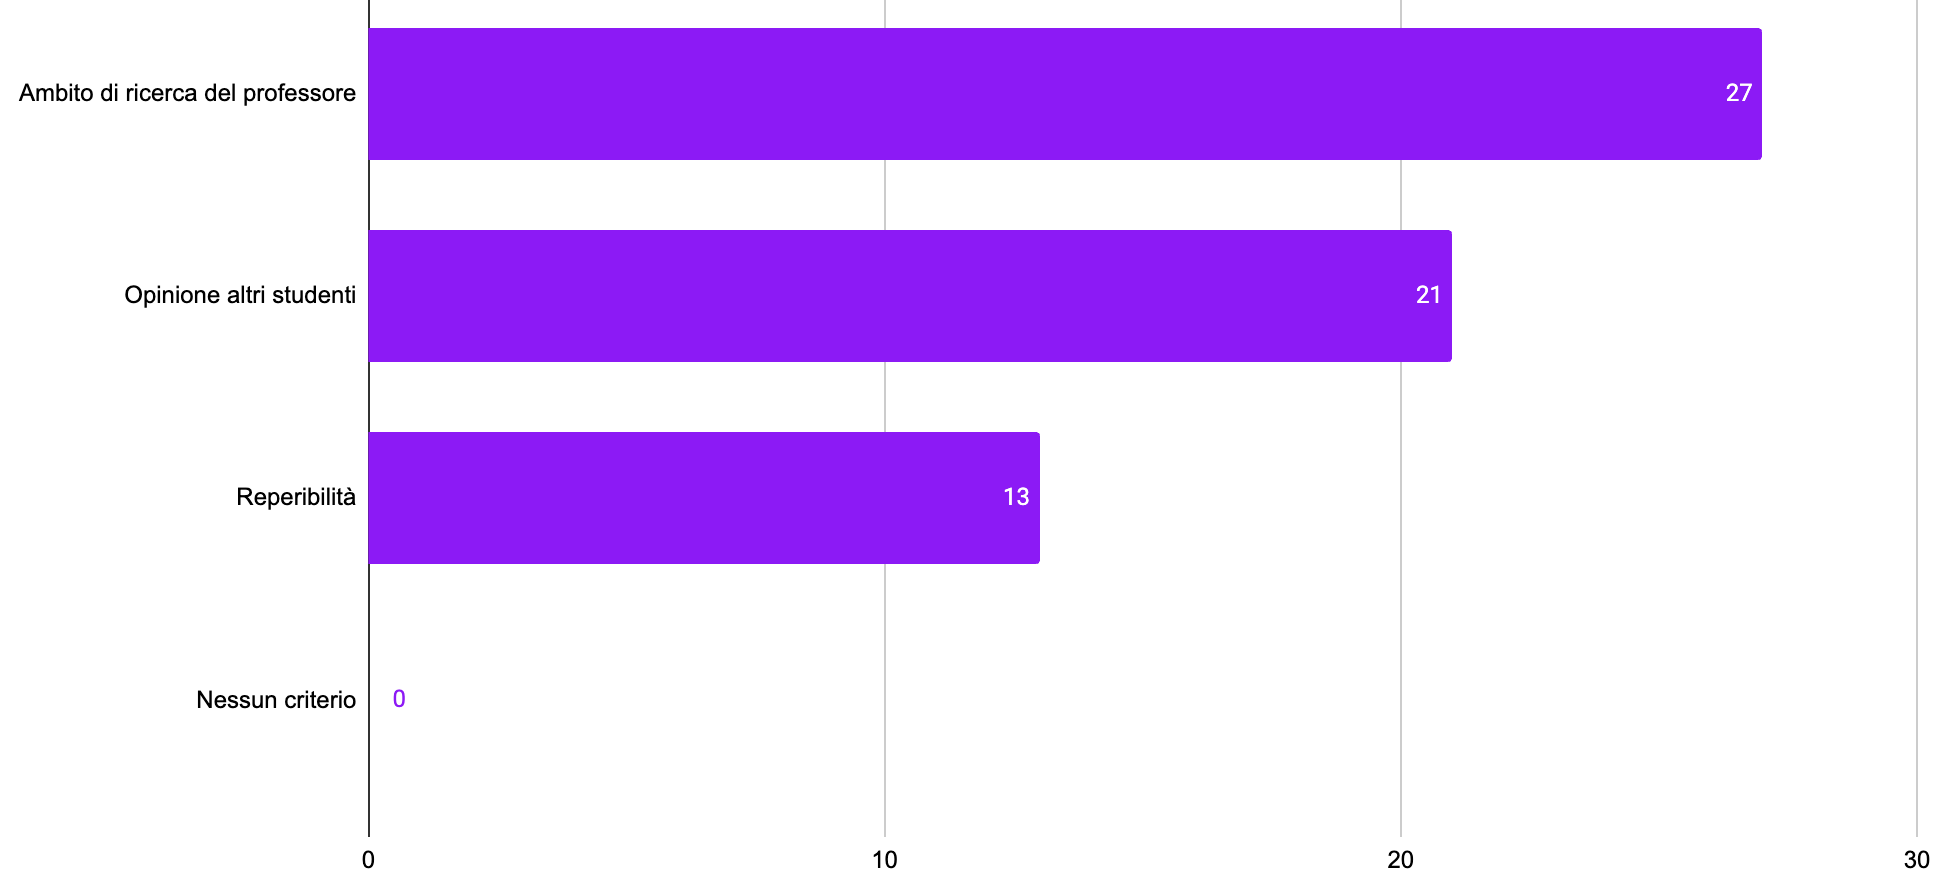
\includegraphics[width=1.0\textwidth]{/Users/leonardvincentramil/Desktop/MyDoc/MyLatex/ProgettoINTRUSIACSAI/01_NeedFinding/img/22.png}
    \end{center}
    \item Quanto i consigli dei tuoi colleghi hanno influenzato la scelts del professore per il tirocinio?
    \begin{center}
        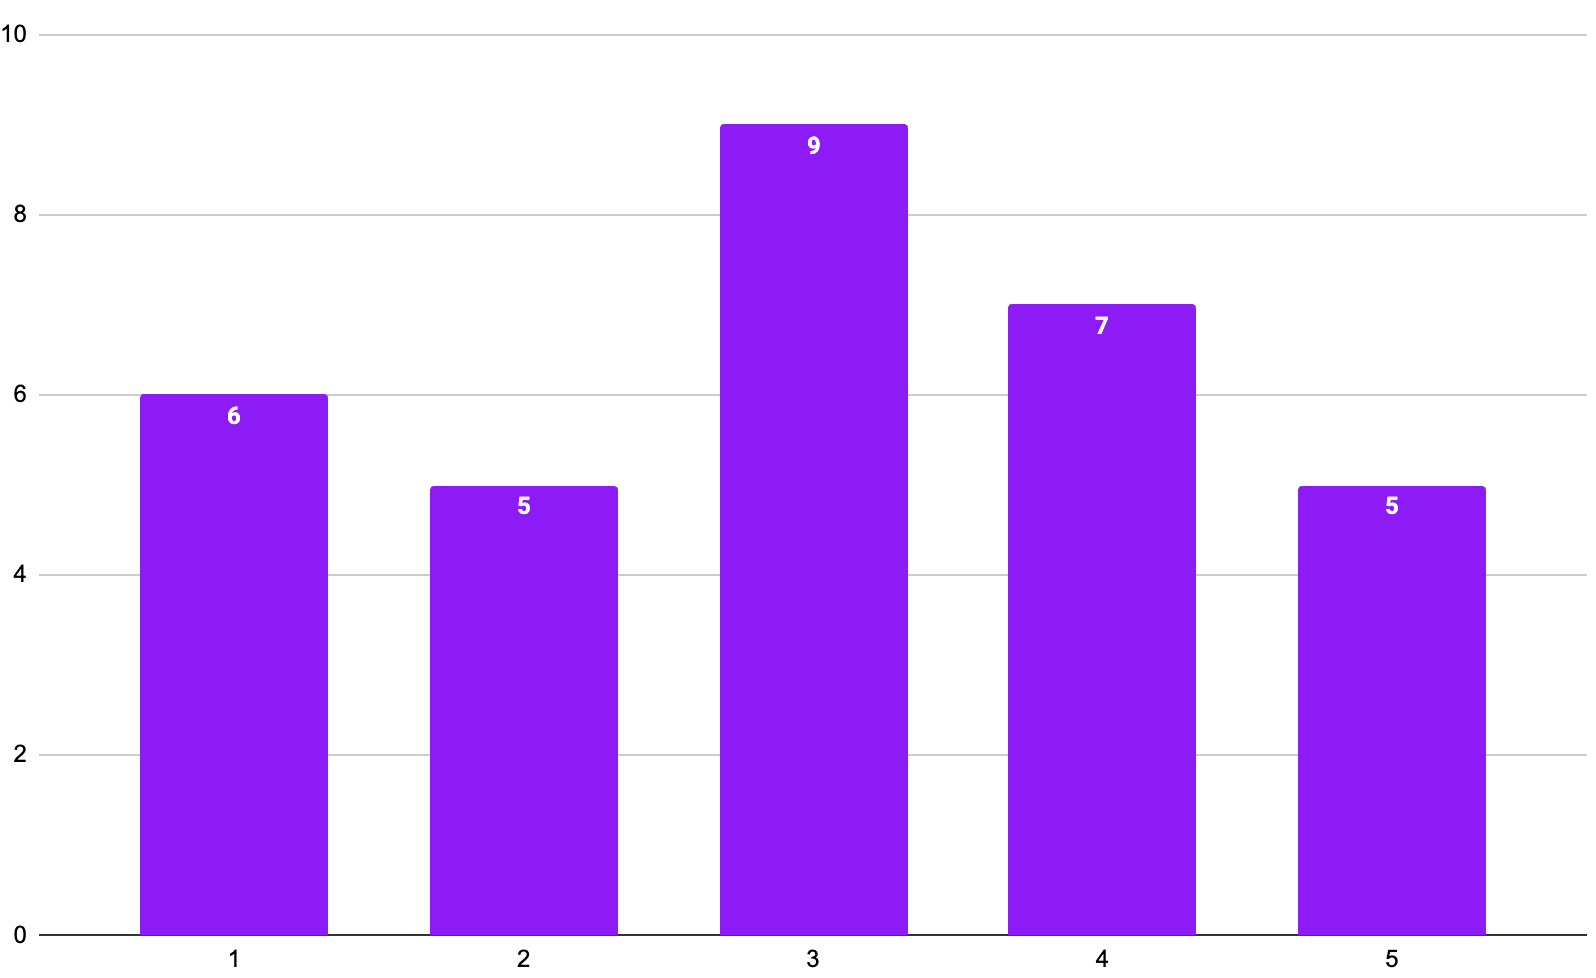
\includegraphics[width=0.8\textwidth]{/Users/leonardvincentramil/Desktop/MyDoc/MyLatex/ProgettoINTRUSIACSAI/01_NeedFinding/img/23.png}
    \end{center}
\end{enumerate}

\subsection{Conclusione Questionario}
A seguito dei risultati ottenuti tramite il questionario, è stato possibile notare come:
\begin{enumerate}
    \item \textbf{Riguardante alla Tematica \textit{Percorso Formativo}}
    \begin{itemize}
        \item Abbiamo avuto un buon numero di persone (ben 73 su 89) che sapevano di avere corsi a scelta nel proprio percorso di studi. 
        Questo ci ha permesso di ottenere risultati più precisi riguardanti le domande del percorso formativo
        \item Ci sia poca chiarezza nei seguenti aspetti:
        \begin{enumerate}
            \item Modificabilità (se si può modificare) (con ben 42 voti)
            \item Tempestiche (con ben 29 voti)
            \item Dove si Compila (con ben 24 voti)
        \end{enumerate}
        Da questi risultati, possiamo notare che:
        \begin{itemize}
            \item vi è la conferma di una delle conclusioni emerse dalle interviste, ossia che
            c'è poca chiarezza sui passaggi e sulle tempistiche riguardanti la compilazione del percorso formativo
            \item emerge un'esigenza di specificare dove effettivamente bisogna compilarlo
        \end{itemize} 
        \item un buon numero di studenti sceglie il piano di studi rispetto a cosa si vuole specializzare, aspetto che è emerso tra le conclusioni delle interviste
        \item un aspetto interessante che non è emerso dalle interviste è l'incompatibilità con l'orario di altri corsi. 
        \item vi è un ulteriore conferma della quale molti studenti scelgono i corsi in base al professore e alla modalità di esame
    \end{itemize}
    \item \textbf{Riguardante alla Tematica \textit{Opinione riguardanti i Professori}}
    \begin{itemize}
        \item I parametri che ricercano gli studenti dai professori sono principalmente:
        \begin{itemize}
            \item Chiarezza durante le Lezioni (77 voti)
            \item Modalità di Esame (69 voti)
            \item Programma che viene svolto (43 voti)
            \item Risorse (43 voti)
        \end{itemize}
        \item al contrario delle interviste, il materiale del professore sia semplice da reperire
        \item sia indispensabile la condivisione dei materiali con i colleghi
    \end{itemize}
    
    \item \textbf{Riguardante alla Tematica \textit{Tirocinio}}
    \begin{itemize}
        \item vi è la conferma di una delle conclusioni emerse dalle interviste, ossia che ci sia poca chiarezza riguardo alle ore da svolgere e l'inizio e fine del tirocinio
        \item sfortunatamente, abbiamo avuto pochi dati da analizzare considerando che soltanto 56 studenti che hanno il tirocinio 34 risultano avere il tirocinio interno.
        \item c'è poca chiarezza riguardante le informazioni del tirocinio
        \item i criteri emersi per scegliere il professore per il tirocinio sono:
        \begin{itemize}
            \item l'ambito di ricerca
            \item l'opinione degli studenti
        \end{itemize}
        \item i consigli dei propri colleghi influenzino non di tanto nella scelta del tirocinio
    \end{itemize}
    
\end{enumerate}

\section{Conclusione}
Per concludere, dopo una dura analisi vi elenchiamo i \textit{Need} con i rispettivi \textit{Task} che siamo riusciti ad individuare:
\begin{enumerate}
    \item \textbf{Gli studenti hanno bisogno di maggiore chiarezza all'interno del sito Sapienza riguardante il tirocinio e il percorso formativo.}\\
     Dalle interviste è infatti emersa la poca chiarezza dei passaggi, delle tempistiche e del dove riguardo alla compilazione sia del percorso formativo che del tirocinio.
    \item \textbf{Necessità di maggiore e più facilitata comunicazione tra studenti per scambio di opinioni riguardo corsi e professori e condivisione di appunti per studiare.}\\
    Gli studenti hanno evidenziato l’esigenza di più comunicazione tra di loro riguardanti materiali e opinioni riguardo i professori. Queste informazioni sono per loro necessarie al fine di scegliere il corso ed i tirocini a loro più adatti.
    \item \textbf{Necessità di avere le informazioni più rilevanti, riguardo ai corsi, a portata di mano, concentrate in un unico posto e facilmente raggiungibili.}\\
    In particolare, nella scelta dei corsi per il percorso formativo, lo studente ha necessità di trovare informazioni come la modalità d’esame, la lingua di erogazione del corso, dove trovare il materiale e la carriera del professore di quel corso ma molto spesso queste informazioni sono sparpagliate.
    \item \textbf{Necessità di poter essere a conoscenza se un particolare corso a scelta è in linea con il percorso formativo da loro originariamente scelto.}\\
     Questo non sempre è possibile per esempio per colpa delle descrizioni poco chiare fornite sul sito Sapienza.
\end{enumerate}

\subsection{Need 1}
\begin{center}
    \textit{Gli studenti hanno bisogno di maggiore chiarezza all'interno del sito Sapienza riguardante il tirocinio e il percorso formativo. Dalle interviste è infatti emersa la poca chiarezza dei passaggi e delle tempistiche riguardo alla compilazione sia del percorso formativo che del tirocinio.}
\end{center}
\subsubsection{Task 1: Tempistiche e passaggi Percorso Formativo}
\begin{enumerate}
    \item Ricercare il nome del Corso di Laurea interessato
    \item Selezionare il Corso di Laurea di interesse
    \item Navigare sul Percorso formativo
    \item Visualizzare le informazioni riguardo passaggi e tempistiche della compilazione dello stesso
\end{enumerate}

\subsubsection{Task 2: Tempistiche e passaggi Tirocinio}
\begin{enumerate}
    \item Ricerca del Corso di Laurea
    \item Selezionare il Corso di Laurea
    \item Navigare sulle modalità di compilazione del tirocinio 
    \item Navigare sulle tempistiche di compilazione del tirocinio
\end{enumerate} 

\subsection{Need 2}
\begin{center}
    \textit{Necessità di maggiore e più facilitata comunicazione tra studenti per scambio di opinioni riguardo corsi e professori e condivisione di appunti per studiare. 
    Gli studenti hanno evidenziato l’esigenza di più comunicazione tra di loro riguardanti materiali e opinioni riguardo i professori. Queste informazioni sono per loro necessarie al fine di scegliere il corso ed i tirocini a loro più adatti.}
\end{center}
\subsubsection{Task 1: Commenti Insegnamenti (corsi)}
\begin{enumerate}
    \item Ricerca dell'insegnamento (corso) di interesse
    \item Selezionare l'insegnamento (corso) interessato
    \item Navigare sui Commenti degli altri utenti per vedere le loro opinioni
\end{enumerate}

\subsubsection{Task 2: Conoscere meglio un Professore}
\begin{enumerate}
    \item Ricercare il nome del professore di tuo interesse
    \item Seleziona il professore desiderato
    \item Visualizza le informazioni di tuo interesse tra quelle disponibili riguardanti il professore
    \item Naviga sulle recensioni e/o sui commenti postati da altri studenti 
    \item Visualizza il suo curriculum vitae 
\end{enumerate}


\subsubsection{Task 3: Condivisione degli Appunti}
\begin{enumerate}
    \item Ricercare il nome del corso desiderato
    \item Selezioni il corso d’interesse
    \item Ricerca l’argomento di quel corso su cui ti servono appunti
    \item Visualizza gli appunti su quell’argomento postati da altri studenti (eventualmente ordinati in base alle recensioni di altri studenti)  
\end{enumerate}

\subsubsection{Task 4: Informarsi sul Tirocinio disponibile del Professore}
\begin{enumerate}
    \item Ricercare il nome del professore di tuo interesse
    \item Seleziona il professore desiderato
    \item Visualizza le informazioni di tuo interesse tra quelle disponibili riguardanti il professore
    \item Naviga sui tirocini disponibili del professore cercato
\end{enumerate} 

\subsection{Need 3}
\begin{center}
    \textit{Necessità di avere le informazioni più rilevanti, riguardo ai corsi, a portata di mano, concentrate in un unico posto e facilmente raggiungibili.
    In particolare, nella scelta dei corsi per il percorso formativo, lo studente ha necessità di trovare informazioni come la modalità d’esame, la lingua di erogazione del corso, dove trovare il materiale e la carriera del professore di quel corso ma molto spesso queste informazioni sono sparpagliate.}
\end{center}
\subsubsection{Task 1: Ottenere le informazioni riguardanti quel particolare corso}
\begin{enumerate}
    \item Ricerca il nome del corso di tuo interesse
    \item Selezionalo
    \item Naviga sulle informazioni del corso
    \item Visualizza le informazioni di tuo interesse, come modalità d’esame, professore del corso, ecc...
\end{enumerate}


\subsection{Need 4}
\begin{center}
    \textit{Gli studenti hanno evidenziato la necessità di poter essere a conoscenza se un particolare corso a scelta è in linea con il percorso formativo da loro originariamente scelto. (Questo non sempre è possibile per esempio per colpa delle descrizioni poco chiare fornite sul sito Sapienza.)    }
\end{center}
\subsubsection{Task 1: Ricerca dei possibili corsi che uno studente può seguire}
\begin{enumerate}
    \item Ricercare il nome del corso di laurea
    \item Seleziona il corso di laurea interessato
    \item Navigare sul Percorso Formativo 
    \item Visualizzare i corsi idonei al percorso formativo / compatibili al Corso di Laurea interessato 
\end{enumerate}

%\textbf{Aggiungere: Task per aggiungere gli appunti}